\documentclass[a4paper,11pt]{article}
\usepackage{jheppub}
\usepackage{bvrshorthand}
\usepackage{tikz}
\usepackage{bbm}
\usepackage{siunitx}
\usepackage{adjustbox}
\usepackage{bbold}
\usepackage{marvosym}
\usepackage{multirow}
\usetikzlibrary{shapes.misc}
\usetikzlibrary{decorations.markings}
\usetikzlibrary{decorations.pathmorphing, patterns,shapes}
\usetikzlibrary{calc,shapes.geometric}
\usepackage[most]{tcolorbox}
\definecolor{lightgray}{gray}{0.9}
\usepackage{graphicx}
\usepackage{subcaption}
\usepackage[T1]{fontenc}
\usepackage[utf8]{inputenc}
\usepackage{lmodern}
\usepackage{amsmath,amssymb,mathtools}
\usepackage{booktabs}
\usepackage{enumitem}
\usepackage{xcolor}
\usepackage{placeins}
\usepackage{array}
\usepackage{caption}

\tikzset{cross/.style={cross out, draw=black, minimum size=2*(#1-\pgflinewidth), inner sep=0pt, outer sep=0pt},
	%default radius will be 1pt. 
	cross/.default={1pt}}

\newcommand{\orange}{\color[rgb]{1,.5,0}}
\newcommand{\blue}{\color[rgb]{0.13,0.67,0.8}}
\newcommand{\MF}[1]{{\blue\bf [MF: #1]}}
\newcommand{\D}{{\Delta}}
\renewcommand{\d}{{\delta}}

\newcommand{\II}{\mathrm{I\!I}}
\newcommand{\Kt}{\widetilde{K}}
\newcommand{\xiscr}{\xi_{\rm scr}}
\newcommand{\dd}{\mathrm{d}}
\newcommand{\chk}{\par\smallskip\noindent\textbf{Check.}\ }
\newcommand{\why}{\par\smallskip\noindent\textbf{Why.}\ }
\newcommand{\pb}[1]{{\color{red!80!black}#1}}
\newcommand{\prob}[1]{\par\smallskip\noindent{\color{red!80!black}\textbf{Problem.}\ #1}\par\smallskip}
	

\newcommand{\sD}{\mathsf{D}}% displacement operator (D is already the dilatation operator)

\begin{document}
	\title{Notes on thermal EFT with defects}



	\author{Maddalena Ferragatta}

	\affiliation{CPHT, CNRS, École Polytechnique, Institut Polytechnique de Paris, 91120 Palaiseau, France}


	\maketitle

		
\section{Introduction}\label{sec:bg}

Consider a conformal defect $\cD$ of dimension $p$. It is an extended operator whose support is a $p$-dimensional submanifold of spacetime. Its codimension is $q=d-p$. We assume that $\cD$ preserves rotations of its transverse directions, and that it is invariant under reversing the orientation of its support.

At zero temperature all directions are equivalent, so there is only one way to place a flat defect. On $S^1_\beta\times S^{d-1}_R$ the thermal circle is singled out, and there are two inequivalent ways to place a defect, which we call the two types, shown in Figure \ref{fig:placements} (see ~\cite{Barrat:2024aoa,Artico:2026rye}).
\begin{itemize}
	\item[(a)] \emph{Localised on the thermal circle.} The support is a closed, smooth submanifold $\Sigma\subset S^{d-1}_R$ of dimension $p$, placed at the single Euclidean time $\tau=0$. The defect does not change the Hilbert space. It is an operator acting on the ordinary Hilbert space of the CFT on $S^{d-1}_R$, inserted in the thermal trace.
	\item[(b)] \emph{Wrapping the thermal circle.} The support is $S^1_\beta\times P$, with $P\subset S^{d-1}_R$ of dimension $p-1$. The defect is present at every Euclidean time: it is a static impurity and changes the Hilbert space on the spatial sphere.
	\end{itemize}

\begin{figure}[!htb]
	\centering
	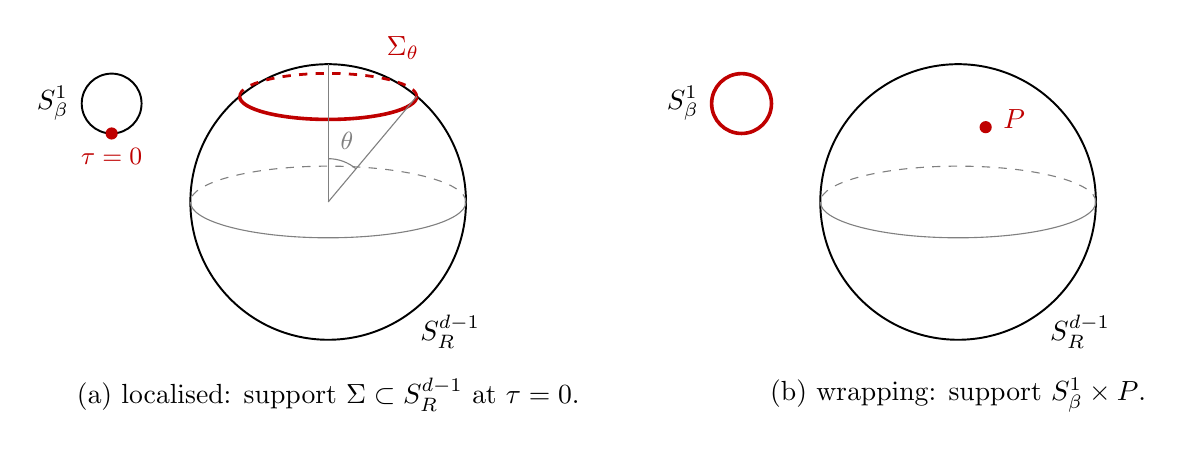
\begin{tikzpicture}[scale=1.0,>=stealth]
		% ---------- panel (b): wrapping ----------
		\begin{scope}[shift={(4.0,0)}]
			\def\r{1.75}
			\draw[line width=0.7pt] (0,0) circle (\r);
			\draw[gray,dashed,line width=0.4pt] (\r,0) arc (0:180:{\r} and {0.26*\r});
			\draw[gray,line width=0.4pt] (-\r,0) arc (180:360:{\r} and {0.26*\r});
			% thermal circle, carrying the defect
			\draw[red!75!black,line width=1.3pt] (-2.75,1.25) circle (0.38);
			\node[left] at (-3.17,1.25) {$S^1_\beta$};
			% P on the sphere
			\fill[red!75!black] (0.35,0.95) circle (2.2pt);
			\node[red!75!black,right] at (0.45,1.05) {$P$};
			\node at (1.55,-1.65) {$S^{d-1}_R$};
			\node at (0,-2.45) {(b) wrapping: support $S^1_\beta\times P$.};
		\end{scope}
		% ---------- panel (a): localised ----------
		\begin{scope}[shift={(-4.0,0)}]
			\def\r{1.75}
			\draw[line width=0.7pt] (0,0) circle (\r);
			\draw[gray,dashed,line width=0.4pt] (\r,0) arc (0:180:{\r} and {0.26*\r});
			\draw[gray,line width=0.4pt] (-\r,0) arc (180:360:{\r} and {0.26*\r});
			% thermal circle with the time tau=0 marked
			\draw[line width=0.7pt] (-2.75,1.25) circle (0.38);
			\fill[red!75!black] (-2.75,0.87) circle (2.2pt);
			\node[left] at (-3.17,1.25) {$S^1_\beta$};
			\node[red!75!black,below] at (-2.75,0.80) {\small $\tau=0$};
			% latitude Sigma_theta at polar angle 40 degrees
			\pgfmathsetmacro{\yc}{\r*cos(40)}
			\pgfmathsetmacro{\xa}{\r*sin(40)}
			\draw[red!75!black,dashed,line width=1.0pt] (\xa,\yc) arc (0:180:{\xa} and {0.26*\xa});
			\draw[red!75!black,line width=1.3pt] (-\xa,\yc) arc (180:360:{\xa} and {0.26*\xa});
			\node[red!75!black] at (0.95,1.95) {$\Sigma_\theta$};
			% polar angle
			\draw[gray,line width=0.4pt] (0,0) -- (0,\r);
			\draw[gray,line width=0.4pt] (0,0) -- (\xa,\yc);
			\draw[gray,line width=0.4pt] (0,0.55) arc (90:50:0.55);
			\node[gray] at (0.24,0.78) {\small $\theta$};
			\node at (1.55,-1.65) {$S^{d-1}_R$};
			\node at (0,-2.45) {(a) localised: support $\Sigma\subset S^{d-1}_R$ at $\tau=0$.};
		\end{scope}
	\end{tikzpicture}
	\caption{The two types of $p$-dimensional defect on $S^1_\beta\times S^{d-1}_R$; the support is drawn in red. (a) The defect sits at one Euclidean time and wraps a $p$-dimensional submanifold of the spatial sphere, here the latitude $\Sigma_\theta$. (b) The defect wraps the thermal circle and sits on a $(p-1)$-dimensional locus $P$ of the sphere.}
	\label{fig:placements}
\end{figure}

\section{Effective theory for a defect at fixed Euclidean time}\label{sec:main}

We consider a conformal field theory on $\mathbb{R}\times S^{d-1}_R$ in the presence of a single conformal defect of dimension $p$ of type (a) of Section~\ref{sec:bg}: its support is $\Sigma\subset S^{d-1}_R$ at fixed Euclidean time, as in Figure~\ref{fig:placements}(a). Finite temperature is introduced by compactifying Euclidean time, which gives $S^1_\beta\times S^{d-1}_R$ with the defect still at $\tau=0$.

A defect of type (a) is an operator on the Hilbert space of the CFT on $S^{d-1}_R$, so we define
\begin{equation}
	Z[\beta]=\Tr\, e^{-\beta D/R}\, ,\qquad
	Z[\beta,\cD]=\Tr\bigl(\cD\, e^{-\beta D/R}\bigr)\, ,\qquad
	W_\beta[\Sigma]\colonequals\log\frac{Z[\beta,\cD]}{Z[\beta]}\, ,
\end{equation}
with $D$ the dilatation operator, so that $D/R$ is the Hamiltonian on the sphere. The first trace is the thermal partition function and the second is the same trace with the defect inserted. Their ratio is the thermal expectation value of $\cD$, and $W_\beta$ is its logarithm. This is the quantity that we expand at high temperature.

\subsection{Set-up and conventions}
We now describe the embedding in $S^{d-1}_R$ of the support $\Sigma$ of the defect. To do that, we need four kinds of indices. Greek indices $\mu,\nu=0,\dots,d-1$ label spacetime, with $x^0=\tau$. Latin indices $i,j,k,l=1,\dots,d-1$ label the spatial slice $S^{d-1}_R$. Indices $a,b,c=1,\dots,p$ label the directions tangent to $\Sigma$, on which we use coordinates $\sigma^a$. Capital indices $A,B=1,\dots,d-1-p$ label the directions normal to $\Sigma$ inside the spatial slice.

We work in Euclidean signature on $S^1_\beta\times S^{d-1}_R$ with $d\ge 3$,
\begin{equation}
	\dd s^2=\dd\tau^2+R^2\,\dd\Omega_{d-1}^2\, ,\qquad \tau\sim\tau+\beta\, ,\qquad \beta=1/T \, .
\end{equation}
The Riemann tensor, Ricci tensor and Ricci scalar of the sphere $S^{d-1}_R$ are
\begin{equation}\label{eq:ambient}
	\cR_{ijkl}=\frac{1}{R^2}\,\bigl(g_{ik}g_{jl}-g_{il}g_{jk}\bigr),\qquad
	\cR_{ij}=\frac{d-2}{R^2}\,g_{ij},\qquad \cR=\frac{(d-1)(d-2)}{R^2}\, ,
\end{equation}
where $g_{ij}$ is its metric. 

The support $\Sigma$ is described by an embedding $\sigma^a\mapsto X^i(\sigma)$ into the spatial slice. Its shape is encoded in two tensors. The first is the induced metric,
\begin{equation}
	\gamma_{ab}=g_{ij}\,\partial_aX^i\partial_bX^j\,  ,
\end{equation}
which measures lengths along $\Sigma$. The second is the second fundamental form, which measures how $\Sigma$ bends inside the spatial slice. It is 
\begin{equation}
	\II^A_{ab}=n^A_i\bigl(\partial_a\partial_bX^i+\Gamma^i_{jk}\,\partial_aX^j\partial_bX^k\bigr)\, ,
\end{equation}
where $\Gamma^i_{jk}$ are the Christoffel symbols of $g_{ij}$ and we introduced $n^A_i$ as an orthonormal set of unit normals to each point of $\Sigma$:
\begin{equation}
	n^A_i\,\partial_aX^i=0,\qquad g^{ij}n^A_in^B_j=\delta^{AB} .
\end{equation}
The second fundamental form has one derivative more than the metric and so carries dimension one. It is useful to separate its trace, the mean curvature vector, from its traceless part:
\begin{equation}
	K^A=\gamma^{ab}\,\II^A_{ab},\qquad\qquad \Kt^A_{ab}=\II^A_{ab}-\tfrac1p\,\gamma_{ab}K^A \, .
\end{equation}
The mean curvature vector measures the average bending, and the traceless part measures how much the bending differs from one tangent direction to another. A submanifold with $\Kt^A_{ab}=0$ bends equally in all directions and is called \emph{umbilic}. Out of these tensors we build the scalars
\begin{equation}\label{eq:scalars}
	K^2\colonequals K^AK_A,\qquad \II^2\colonequals\II^A_{ab}\II_A^{ab},\qquad \Kt^2\colonequals\Kt^A_{ab}\Kt_A^{ab}=\II^2-\tfrac1p K^2 .
\end{equation}
We denote by $\nabla_a$ the covariant derivative along $\Sigma$ and by $R_\Sigma$ the intrinsic Ricci scalar of $\gamma_{ab}$. The latter is not independent of the quantities above: the Gauss equation gives
\begin{equation}\label{eq:gauss}
	R_\Sigma=\gamma^{ac}\gamma^{bd}\cR_{abcd}+K^2-\II^2\, ,
\end{equation}
where $\cR_{abcd}\colonequals\cR_{ijkl}\,\partial_aX^i\partial_bX^j\partial_cX^k\partial_dX^l$. In our case the spatial slice is the round sphere $S^{d-1}_R$, and the Gauss equation simplifies for any $\Sigma$ of dimension $p$ inside it. Substituting equations \eqref{eq:ambient} and \eqref{eq:scalars} it becomes
\begin{equation}\label{eq:gausssphere}
R_\Sigma= \frac{p(p-1)}{R^2}+\Bigl(1-\frac1p\Bigr)K^2-\Kt^2\, .
\end{equation} 
For a line, $p=1$, these formulas simplify: $\II^A=K^A$ is the curvature vector $K^i$ of \cite{BMP}, $\Kt=0$ and $R_\Sigma=0$.

Most explicit formulas below refer to one family of shapes, which we are going to refer to as ``the latitude $S^p$''. To obtain it, let us embed $S^{d-1}_R\subset\mathbb{R}^d$, pick a unit vector $n_0$ and a $(p+1)$-plane orthogonal to it, and set
\begin{equation}\label{eq:lat}
	\Sigma_\theta:\qquad X=R\,\bigl(\cos\theta\,n_0+\sin\theta\,\hat y\bigr),\qquad \hat y\in S^p\subset\mathbb{R}^{p+1},\qquad 0<\theta<\pi .
\end{equation}
This is a round $p$-sphere of radius $R\sin\theta$ at polar angle $\theta$ from $n_0$, drawn in Figure~\ref{fig:placements}(a). The latitude exists for $p\le d-2$.

Its induced metric is $\gamma_{ab}=R^2\sin^2\theta\,\hat\gamma_{ab}$, where $\hat\gamma_{ab} \colonequals \partial_a \hat y \partial_b \hat y$ is the induced metric of the unit $S^p$. 

Its geometric data are (see appendix \ref{appAgeom})
\begin{equation}\label{eq:latdata}
	\begin{gathered}
		\mathrm{Vol}(\Sigma_\theta)=\Omega_p\,(R\sin\theta)^p\, ,\qquad
		\II^{\theta}_{ab}=-\frac{\cot\theta}{R}\,\gamma_{ab},\qquad \II^{A\neq\theta}_{ab}=0\, ,\\
		K^2=\frac{p^2\cot^2\theta}{R^2}\, ,\qquad \Kt^2=0\, ,\qquad \nabla_a\II^A_{bc}=0\, ,\qquad R_\Sigma=\frac{p(p-1)}{R^2\sin^2\theta}\, ,
	\end{gathered}
\end{equation}
where $\Omega_p=2\pi^{\frac{p+1}{2}}/\Gamma\bigl(\tfrac{p+1}{2}\bigr)$ is the volume of the unit $S^p$. The latitude is umbilic and all its invariants are constant.

\subsection{The effective theory}\label{sec:eft}

We now construct the high-temperature expansion of $W_\beta[\Sigma]$ showing how locality, dimensional analysis and the symmetries of the defect fix its form up to a few numbers.

\subsubsection{Screening and locality}\label{sec:screening}

In this section we expand on the discussion of \cite{BMP}, explaining under which assumptions the contribution of the defect to the free energy is local on $\Sigma$ at high temperature.

Let us expand every field in Fourier (Matsubara) modes around the thermal circle,
\begin{equation}
	\phi(\tau,x)=\sum_{n\in\mathbb{Z}}\phi_n(x)\,e^{2\pi i n\tau/\beta} \, .
\end{equation}
A derivative along $\tau$ multiplies $\phi_n$ by $2\pi i n/\beta$, so the kinetic term $(\partial_\tau\phi)^2$ becomes a mass term: from the point of view of the spatial slice, $\phi_n$ is a field of mass $2\pi|n|/\beta$. The modes with $n\neq0$ are therefore heavy in any theory, and the correlations that they carry die off over a distance of order $\beta$ or shorter.

The zero modes are the only ones that get no mass from the thermal circle, and what happens to them depends on the theory. If they stay massless, the correlations that they carry decay only as a power of the distance, for instance as $1/x^{d-3}$ for a free scalar in $d\ge4$. We assume instead that the $n=0$ modes are gapped as well, by a thermal mass. Then all correlations are short range, and connected correlation functions in the presence of the defect decay exponentially,
\begin{equation}\label{eq:screen}
	\langle \mathcal{O}(x)\,\mathcal{O}(0)\,\cD\rangle_c\sim e^{-x/\xiscr}\, ,
\end{equation}
where the screening length $\xiscr$ is set by the lightest mode. A conformal theory has no other scale at distances much shorter than $R$, so $\xiscr$ is a number times $\beta$. This holds also for a defect at a single $\tau$, which is a delta function on the thermal circle and therefore sources all the modes, not only $n=0$: each mode responds only within its own range.

The defect enters this assumption in two ways, and it is useful to state them. First, the defect can have its own degrees of freedom, which live on $\Sigma$ and propagate only along it. An extreme example is a defect that hosts a decoupled $p$-dimensional theory. The correlations of these degrees of freedom are not controlled by the thermal mass of the bulk fields, and we assume that they are short range as well. The screening length $\xiscr$ is then the largest of the correlation lengths, in the bulk and on the defect. Second, we assume that the defect disturbs the thermal state only in its neighbourhood: the expectation value of a local operator at a distance $x$ from $\Sigma$ approaches its thermal value as $e^{-x/\xiscr}$. Both statements are true for the defects of Section~\ref{sec:tests}, but they can fail, as we discuss in Section~\ref{sec:summary}.

Correlations are therefore exponentially small beyond the distance $\xiscr$. Let us see how this makes the contribution of the defect local.

Let $\ell_\Sigma$ be the scale below which the defect looks flat. It is the smallest of the lengths that characterise the geometry: the radii of curvature of $\Sigma$, the distance over which its curvature changes, and the radius $R$ of the sphere. We claim that when
\begin{equation}\label{eq:hier}
	\ell_\Sigma\gg\xiscr\, ,
\end{equation}
$W_\beta[\Sigma]$ is given by an expansion in powers of $\xiscr/\ell_\Sigma$, each term of which is an integral over $\Sigma$ of a local geometric scalar, up to a functional of $\Sigma$ that does not depend on $\beta$ and whose variation is local.


To see this, consider that the defect is an operator that does not depend on $\beta$, so differentiating the two traces in the definition of $W_\beta[\Sigma]$ we find
	\begin{equation}\label{eq:dbetamain}
		\partial_\beta W_\beta[\Sigma]=-\bigl(\langle H\rangle_{\cD}-\langle H\rangle\bigr)\, .
	\end{equation}
	Here $H=D/R$ is the Hamiltonian, which is the integral over the sphere of the energy density operator $\varepsilon(x)$
	\begin{equation}
		H=\int_{S^{d-1}_R}\dd^{d-1}x\sqrt g\;\varepsilon(x)\, ,
	\end{equation} 
	and for any operator $\mathcal{O}$ we denote by
	\begin{equation}\label{eq:vevs}
		\langle\mathcal{O}\rangle_{\cD}\colonequals\frac{\Tr\bigl(\cD\,\mathcal{O}\,e^{-\beta H}\bigr)}{\Tr\bigl(\cD\,e^{-\beta H}\bigr)}\, ,\qquad\qquad
		\langle\mathcal{O}\rangle\colonequals\frac{\Tr\bigl(\mathcal{O}\,e^{-\beta H}\bigr)}{\Tr\,e^{-\beta H}}\, ,
	\end{equation}
	its thermal expectation values with and without the defect. 
	Since $H$ is conserved, $\varepsilon(x)$ can be inserted at any Euclidean time, and we choose a time $\tau_0\neq0$, so that it does not sit on the defect. We then define the function
	\begin{equation}\label{eq:calE}
		\mathcal{E}(x)\colonequals\langle\varepsilon(x)\rangle_{\cD}-\langle\varepsilon(x)\rangle\, ,
	\end{equation}
	which is the energy density that the defect adds to the thermal state at the point $x$ of the sphere. With this definition \eqref{eq:dbetamain} becomes
	\begin{equation}\label{eq:dbetaE}
		\partial_\beta W_\beta[\Sigma]=-\int_{S^{d-1}_R}\dd^{d-1}x\sqrt g\;\mathcal{E}(x)\, .
	\end{equation}
	
	Because of screening, $\mathcal{E}(x)$ is exponentially small when the distance of $x$ from $\Sigma$ is larger than $\xiscr$, so only a neighbourhood of $\Sigma$ contributes to \eqref{eq:dbetaE}. In this neighbourhood we label a point $x$ by the nearest point $\sigma$ of $\Sigma$ and by its displacement $y^A$ from it along the normals, $x=(\sigma,y)$. The volume element of the sphere is then
	\begin{equation}\label{eq:tube}
		\dd^{d-1}x\sqrt g=\dd^p\sigma\sqrt\gamma\;\dd^{\,d-1-p}y\;J(\sigma,y)\, ,\qquad\qquad J(\sigma,0)=1\, ,
	\end{equation}
	where $J$ is the Jacobian of the change of coordinates. Integrating first over $y$ we define
	\begin{equation}\label{eq:edef}
		e(\sigma)\colonequals\int\dd^{\,d-1-p}y\;J(\sigma,y)\,\mathcal{E}(\sigma,y)\, ,
	\end{equation}
	which is the energy added by the defect per unit volume of $\Sigma$ at the point $\sigma$. The integral over $y$ converges within a distance of order $\xiscr$, and \eqref{eq:dbetaE} becomes
	\begin{equation}\label{eq:edens}
		\partial_\beta W_\beta[\Sigma]=-\int_\Sigma\dd^p\sigma\sqrt\gamma\;e(\sigma)\, .
	\end{equation}
	
	The shape of $\Sigma$ enters through $e(\sigma)$, and we now show that $e(\sigma)$ depends only on the geometry around $\sigma$. Suppose that we deform $\Sigma$ by a small displacement $\delta X^A$ along its normals. The response to such a deformation defines the displacement operator $\sD_A$ on $\Sigma$ and the definition \eqref{eq:calE} gives
	\begin{equation}\label{eq:deltaE}
		\delta\mathcal{E}(x)=-\int_\Sigma\dd^p\sigma'\sqrt\gamma\;\bigl\langle\varepsilon(x)\,\sD_A(\sigma')\bigr\rangle_{\cD,c}\;\delta X^A(\sigma')\, .
	\end{equation}
	Because of screening this correlator is short range,
	\begin{equation}\label{eq:screenED}
		\bigl\langle\varepsilon(x)\,\sD_A(\sigma')\bigr\rangle_{\cD,c}\sim e^{-r/\xiscr}\, ,
	\end{equation}
	with $r$ the distance between $x$ and the point $X(\sigma')$ of the defect. By \eqref{eq:edef}, a deformation of $\Sigma$ at a distance $r\gg\xiscr$ from $\sigma$ changes $e(\sigma)$ only by a term of order $e^{-r/\xiscr}$. The same is true for a change of the metric of the sphere, with the stress tensor in place of the displacement operator. Hence $e(\sigma)$ depends on the geometry only within a distance of order $\xiscr$ from $\sigma$.
	
	By \eqref{eq:hier} the geometry varies little over this distance, so we can expand the embedding and the metric of the sphere around $\sigma$. At leading order the defect is flat, and so is the space around it. The corrections involve the second fundamental form and the curvature of the sphere, and then their derivatives, all evaluated at $\sigma$. Since $e(\sigma)$ is a scalar, the result is a sum over the local geometric scalars $O_I(\sigma)$ that can be built from them,
	\begin{equation}\label{eq:eexp}
		e(\sigma)=\sum_I\hat e_I(\beta)\;O_I(\sigma)\, ,
	\end{equation}
	where the first scalar is $O_0=1$ and the coefficients $\hat e_I(\beta)$ do not depend on the shape of $\Sigma$. Each derivative of the embedding is of order $1/\ell_\Sigma$ and is multiplied by a distance of order $\xiscr$, so it costs one power of $\xiscr/\ell_\Sigma$.
	
	Inserting \eqref{eq:eexp} in \eqref{eq:edens} and integrating over $\beta$ we find
	\begin{equation}\label{eq:Wloc}
		W_\beta[\Sigma]=C[\Sigma]+\sum_I c_I(\beta)\int_\Sigma\dd^p\sigma\sqrt\gamma\;O_I(\sigma)\, ,\qquad\qquad \partial_\beta c_I(\beta)=-\hat e_I(\beta)\, .
	\end{equation}
	The second equation fixes each $c_I(\beta)$ up to an additive constant, and $C[\Sigma]$ is a functional of $\Sigma$ that does not depend on $\beta$.
	
The functional $C[\Sigma]$ is not arbitrary, because its variation is local as well. Since $Z[\beta]$ does not depend on $\Sigma$, the definition of the displacement operator gives
	\begin{equation}\label{eq:dispW}
		\delta W_\beta[\Sigma]=-\int_\Sigma\dd^p\sigma\sqrt\gamma\;\langle \sD_A(\sigma)\rangle_{\cD}\;\delta X^A(\sigma)\, .
	\end{equation}
	The one-point function $\langle\sD_A(\sigma)\rangle_{\cD}$ depends only on the geometry around $\sigma$, for the same reason as $e(\sigma)$. Comparing \eqref{eq:dispW} with the variation of \eqref{eq:Wloc}, the variation of $C[\Sigma]$ is the part of \eqref{eq:dispW} that does not depend on $\beta$, and it is local as well:
	\begin{equation}\label{eq:deltaC}
		\delta C[\Sigma]=-\int_\Sigma\dd^p\sigma\sqrt\gamma\;E_A(\sigma)\,\delta X^A(\sigma)\, ,
	\end{equation}
	where $E_A(\sigma)$ is a vector normal to $\Sigma$, which is built from the second fundamental form, the curvature of the sphere and their derivatives at $\sigma$, and does not depend on $\beta$. 


The zero modes are the only possible obstruction to this argument, since the modes with $n\neq0$ are short range in any theory. If the zero modes are massless, the correlators decay only as a power law. Points far apart on $\Sigma$ remain correlated, and $W_\beta[\Sigma]$ receives contributions that depend on the global shape of $\Sigma$ and are not integrals of local scalars. A gap is not enough by itself: the hierarchy \eqref{eq:hier} requires $\xiscr\ll\ell_\Sigma$, and $\ell_\Sigma$ is at most $R$.

We expect screening in generic interacting theories, where the interactions give the zero modes a thermal mass. It can fail, however. A free scalar with periodic boundary conditions is not screened (see \cite{BMP}, Section~4.1): in flat space its $n=0$ mode is massless. On the sphere the curvature coupling gives this mode a mass of order $1/R$, but then $\xiscr$ is of order $R$ and \eqref{eq:hier} cannot hold. This is why all tests of the effective theory in the next section use fields that are antiperiodic around the thermal circle. For such fields the frequencies are $(2n+1)\pi/\beta$, so every mode has a mass of at least $\pi/\beta$ and correlation functions decay on the scale $\beta/\pi$.


\subsubsection{The derivative expansion}\label{sec:derexp}

In the previous section we saw that, when $\ell_\Sigma\gg\xiscr$, $W_\beta[\Sigma]$ is the sum \eqref{eq:Wloc} of two parts: integrals of local geometric scalars, with coefficients that depend on $\beta$, and a functional $C[\Sigma]$ that does not depend on $\beta$ and whose variation is local. In this section we classify the scalars, we find how their coefficients depend on $\beta$, and we determine $C[\Sigma]$.

Let us first list the building blocks. A local geometric scalar on $\Sigma$ is built from the second fundamental form $\II^A_{ab}$, from the Riemann tensor of the spatial slice and its covariant derivatives, projected on the directions tangent and normal to $\Sigma$, and from the covariant derivative $\nabla_a$ along $\Sigma$. The indices are contracted with $\gamma^{ab}$ and $\delta_{AB}$. To each scalar we assign its dimension $n$ in units of inverse length: $\II^A_{ab}$ and $\nabla_a$ have dimension one, and the Riemann tensor has dimension two. Let $O_{n,I}$ be the independent scalars of dimension $n$, labelled by $I$. These are the scalars $O_I$ of the previous section, now organised by their dimension, and we call $c_{n,I}(\beta)$ the corresponding coefficients $c_I(\beta)$. The result \eqref{eq:Wloc} of the previous section then reads
\begin{equation}\label{eq:localform}
	W_\beta[\Sigma]= C[\Sigma]+\sum_{n,I}c_{n,I}(\beta)\int_\Sigma\dd^p\sigma\sqrt\gamma\;O_{n,I}\, ,
\end{equation}
where the coefficients $c_{n,I}(\beta)$ do not depend on the shape of $\Sigma$.
By \eqref{eq:Wloc}, each one is fixed by $\partial_\beta c_{n,I}=-\hat e_{n,I}$ up to an additive constant. The coefficient $\hat e_{n,I}$ comes from distances of order $\xiscr$, where the defect and the space around it are flat, so it is fixed by the theory in flat space at temperature $1/\beta$. It is finite, because the energy density in \eqref{eq:calE} sits at $\tau_0\neq0$, away from the defect. The only length it can depend on is $\beta$, and by dimensional analysis $\hat e_{n,I}=\beta^{\,n-p-1}\times\text{(a number)}$. Integrating over $\beta$ gives $\beta^{\,n-p}$ for $n\neq p$ and $\log\beta$ for $n=p$, plus a constant.
	
	The constant does not depend on $\beta$, and not on $R$ either, since $R$ enters only through the curvature, which is already in $O_{n,I}$. So for $n\neq p$ it is a number times $\epsilon^{\,n-p}$, with $\epsilon$ the short-distance cutoff. For $n>p$ it vanishes as $\epsilon\to0$. For $n<p$ it is a power divergence, which is removed by a counterterm that is local on $\Sigma$ and does not depend on the temperature, as in \cite{BMP}. Hence, for $n\neq p$,
	\begin{equation}\label{eq:cscaling}
		c_{n,I}(\beta)=\beta^{\,n-p}\times\text{(a number)}\, .
	\end{equation}
	For $n=p$ the constant is a number that does not depend on $\beta$, so its term is part of $C[\Sigma]$, and the sum in \eqref{eq:localform} is over $n\neq p$. The logarithm appears as $\log(\beta/\epsilon)$. It is a logarithmic divergence, and it cannot be removed by a counterterm because it depends on $\beta$. It exists only for even $p$, since for odd $p$ there is no scalar of dimension $p$. We treat it in section \ref{sec:log} and ignore it in the rest of this section.


Next we note that only even $n$ appear in \eqref{eq:localform}. To see this, observe that each building block has a number of indices with the same parity as its dimension: $\II^A_{ab}$ has three indices and dimension one, $\nabla_a$ has one index and dimension one, the Riemann tensor has four indices and dimension two, and each covariant derivative acting on it adds one index and one unit of dimension. A scalar is obtained by contracting all the indices in pairs, so it contains an even number of indices and has even dimension.

This counting fails only for a scalar that is built with an $\varepsilon$-tensor, either the one of $\Sigma$ or the one of the directions normal to $\Sigma$ inside the slice. Neither can appear. 
	
	Indeed, a scalar that contains only the $\varepsilon$-tensor of $\Sigma$ changes sign when the orientation of $\Sigma$ is reversed, and it is excluded because we assumed that the defect is invariant under this operation.
	
	On the other hand, a scalar that contains the $\varepsilon$-tensor of the spatial slice changes sign when $\Sigma$ is replaced by its mirror image $P\Sigma$, with $P$ a reflection of the sphere. An example is the torsion of a line in $d=4$, which measures how the line twists like a helix. It does not depend on the orientation of the line, so it is not excluded by the previous argument, but a left-handed helix becomes right-handed in a mirror. However, such a scalar is excluded because $W_\beta[P\Sigma]=W_\beta[\Sigma]$. To see this, consider the map $(\tau,x)\to(-\tau,Px)$. It is an isometry of $S^1_\beta\times S^{d-1}_R$, and it preserves the orientation of spacetime, because it reverses both the direction of $\tau$ and the orientation of the sphere. A theory on a curved space depends only on the metric and on the orientation, so this map is a symmetry. It keeps the defect at $\tau=0$ and moves its support from $\Sigma$ to $P\Sigma$. Since the defect is invariant under rotations of its transverse directions and under reversing its orientation, no other data are needed to specify it, and the map sends it to the same defect on $P\Sigma$.


It remains to determine $C[\Sigma]$. By \eqref{eq:deltaC} its variation is given by a vector $E_A$ normal to $\Sigma$, built from the same building blocks as the scalars, with coefficients that are numbers because it does not depend on $\beta$. Since $C[\Sigma]$ is dimensionless and $\dd^p\sigma\sqrt\gamma\,\delta X^A$ has dimension $-(p+1)$, the vector $E_A$ has dimension $p+1$. On the other hand, $E_A$ has one free index, so by the counting of the indices above its dimension is odd.

For odd $p$ this is impossible, so $E_A=0$: $C[\Sigma]$ does not change when $\Sigma$ is deformed, and we call it $\gamma[\cD]$. For even $p$ the vector $E_A$ can be different from zero, because the integrals of the scalars of dimension $p$ have a variation of this form. We claim that they are the only terms of $C[\Sigma]$ that depend on the shape of $\Sigma$:
\begin{equation}\label{eq:Cloc}
	C[\Sigma]=\gamma[\cD]+\sum_I k_I\int_\Sigma\dd^p\sigma\sqrt\gamma\;O_{p,I}\, ,
\end{equation}
with numbers $k_I$. For $p=2$ we prove this in Appendix~\ref{app:local}. For even $p\ge4$ we expect it to hold as well, but we do not prove it here: the argument of Appendix~\ref{app:local} has to be supplemented by a classification of more terms of $E_A$.

The term $\gamma[\cD]$ does not change when $\Sigma$ is deformed smoothly. It can therefore depend only on the topology of $\Sigma$ and, when the codimension of $\Sigma$ in the sphere is small, on the way in which $\Sigma$ is knotted. For $d-1\geq 2p+2$ there are no knots, and only the topology is left.

The integrals in \eqref{eq:Cloc} are the terms with $n=p$ that were missing in \eqref{eq:localform}, with $c_{p,I}=k_I$. We conclude that
\begin{equation}\label{eq:Wloc2}
	W_\beta[\Sigma]=\gamma[\cD]+\sum_{n,I}c_{n,I}(\beta)\int_\Sigma\dd^p\sigma\sqrt\gamma\;O_{n,I}\, ,
\end{equation}
where \eqref{eq:cscaling} now holds for every $n$. The numbers in \eqref{eq:cscaling} and $\gamma[\cD]$ are the \emph{Wilson coefficients} of the effective theory: they depend on the CFT and on the defect, but not on $\Sigma$, $\beta$ or $R$.

Collecting the scalars of dimension $n$ in a single combination $\mathcal{L}_n$, with numerical coefficients, we arrive at
\begin{equation}\label{eq:derexp}
	W_\beta[\Sigma]=\gamma[\cD]+\int_\Sigma \frac{\dd^p\sigma\sqrt{\gamma}}{\Omega_p\,\beta^{p}}\,\sum_{n\ge0}\beta^{n}\,\mathcal{L}_n \, .
\end{equation}
The factor $1/\Omega_p$ is a convention for the normalisation of the Wilson coefficients.


Let us now go through the first orders. At $n=0$ the only scalar is a constant, $\mathcal{L}_0=m_D$. The leading term of \eqref{eq:derexp} is then proportional to the volume of the defect,
\begin{equation}
	W_\beta[\Sigma]=\gamma[\cD]+\frac{m_D}{\Omega_p\,\beta^{p}}\,\mathrm{Vol}(\Sigma)+\dots\, .
\end{equation}
For a flat defect in flat space this is the complete answer, since all the other scalars vanish. The number $m_D$ plays the role of a tension: $m_D/(\Omega_p\beta^p)$ is the value of $W_\beta$ per unit volume of a flat defect.

At $n=2$ a scalar is either quadratic in $\II^A_{ab}$ or linear in the Riemann tensor. A single derivative $\nabla_a\II^A_{bc}$ cannot be used, because its normal index has nothing to be contracted with. In a scalar quadratic in $\II^A_{ab}$ the two normal indices are contracted with each other, and the four tangent indices can be contracted in two inequivalent ways. This gives $K^AK_A$ and $\II^A_{ab}\II_A^{ab}$, or equivalently $K^AK_A$ and $\Kt^A_{ab}\Kt_A^{ab}$ by \eqref{eq:scalars}. In a scalar linear in the Riemann tensor, $\cR_{ijkl}$ is contracted with two projectors, each of which is either the tangent projector $\gamma^{ij}\colonequals\gamma^{ab}\partial_aX^i\partial_bX^j$ or the normal projector $g^{ij}-\gamma^{ij}$. The possible choices are tangent--tangent, tangent--normal and normal--normal, which gives three scalars. The intrinsic curvature $R_\Sigma$ is not an additional scalar, because of the Gauss equation \eqref{eq:gauss}. The complete list at $n=2$ is therefore
\begin{equation}\label{eq:L2}
	\mathcal{L}_2=t_2\,K^AK_A+\tilde t_2\,\Kt^A_{ab}\Kt_A^{ab}
	+r_2^{(1)}\,\cR+r_2^{(2)}\,\gamma^{ab}\cR_{ab}+r_2^{(3)}\,\gamma^{ac}\gamma^{bd}\cR_{abcd} \, ,
\end{equation}
with $\cR_{ab}\colonequals\cR_{ij}\,\partial_aX^i\partial_bX^j$. It contains five Wilson coefficients. The coefficient $t_2$ multiplies the square of the mean curvature. It is the first term that distinguishes different shapes, and it plays the role of a bending rigidity. The coefficient $\tilde t_2$ measures the cost of bending by different amounts in different directions. Its term vanishes identically for $p=1$, and on any umbilic $\Sigma$. The coefficients $r_2^{(1)}$, $r_2^{(2)}$ and $r_2^{(3)}$ measure the response of the defect to the curvature of the space in which it sits, and their terms vanish in flat space.

The three curvature scalars are independent on a generic spatial manifold, except that the third one vanishes identically for $p=1$. Moreover, for $p=d-2$ the defect has only one normal direction inside the slice. The normal--normal scalar then vanishes, and the three scalars are related by
\begin{equation}
	\cR-2\,\gamma^{ab}\cR_{ab}+\gamma^{ac}\gamma^{bd}\cR_{abcd}=0\, .
\end{equation}
They are therefore independent only for $2\le p\le d-3$. On the round sphere $S^{d-1}_R$ they are all constants proportional to $1/R^2$. Only the combination
\begin{equation}\label{eq:r2}
	r_2\colonequals(d-1)(d-2)\,r_2^{(1)}+p(d-2)\,r_2^{(2)}+p(p-1)\,r_2^{(3)}
\end{equation}
can then be measured, and \eqref{eq:L2} becomes
\begin{equation}\label{eq:L2sphere}
	\mathcal{L}_2=t_2\,K^2+\tilde t_2\,\Kt^2+\frac{r_2}{R^2}\, .
\end{equation}
Let us finally consider $n=4$. We restrict to the round sphere, where the Riemann tensor is given by \eqref{eq:ambient} and its covariant derivative vanishes. A scalar is then quartic in $\II^A_{ab}$, or it contains two powers of $\II^A_{ab}$ and two derivatives, or it is one of the scalars that we already found, $K^2$, $\Kt^2$ and a constant, multiplied by the appropriate power of $1/R^2$.

In a scalar quartic in $\II^A_{ab}$ the four normal indices are contracted in two pairs, and the eight tangent indices can be contracted in several ways. It is convenient to write $\II^A_{ab}$ in terms of $K^A$ and $\Kt^A_{ab}$. One finds eight scalars: one with four powers of $K^A$, two with two powers, one with one power, and four that contain only $\Kt^A_{ab}$.

In a scalar with two derivatives we can integrate by parts, so that each derivative acts on a different $\II^A_{ab}$. On the sphere the Codazzi equation says that $\nabla_a\II^A_{bc}$ is symmetric in its three tangent indices, so there are only two scalars, $\nabla_a\II^A_{bc}\nabla^a\II_A^{bc}$ and $\nabla_aK^A\nabla^aK_A$. They are not independent, because their integrals differ by terms without derivatives:
\begin{equation}\label{eq:simons}
	\begin{aligned}
		\int_\Sigma\!\dd^p\sigma\sqrt\gamma\;\nabla_a\II^A_{bc}\nabla^a\II_A^{bc}
		={}&\int_\Sigma\!\dd^p\sigma\sqrt\gamma\;\nabla_aK^A\nabla^aK_A
		+\int_\Sigma\!\dd^p\sigma\sqrt\gamma\;\Bigl[-\frac{p\,\Kt^2}{R^2}-K_B\,\mathrm{tr}\bigl(\II^B\II^A\II_A\bigr)\\
		&+2\,\mathrm{tr}\bigl(\II^A\II_A\II^B\II_B\bigr)-2\,\mathrm{tr}\bigl(\II^A\II^B\II_A\II_B\bigr)+\bigl(\II_A\!\cdot\!\II_B\bigr)\bigl(\II^A\!\cdot\!\II^B\bigr)\Bigr]\, .
	\end{aligned}
\end{equation}
Here a dot denotes the contraction of the tangent indices, $\II_A\!\cdot\!\II_B\colonequals\II_{A\,ab}\,\II_B^{ab}$, and $\mathrm{tr}$ is the trace of a product of matrices with tangent indices, $\mathrm{tr}(\II^A\II^B\cdots)\colonequals\II^{A}{}_{a}{}^{b}\,\II^{B}{}_{b}{}^{c}\cdots$. We use the same notation for $\Kt^A_{ab}$. To obtain \eqref{eq:simons} one uses the Codazzi equation, integrates by parts, and commutes two covariant derivatives. The commutator gives the curvature of $\Sigma$ and of its normal bundle, which are quadratic in $\II^A_{ab}$ by the Gauss equation. We keep $\nabla_aK^A\nabla^aK_A$.

The complete list at $n=4$ on the sphere is therefore
\begin{equation}\label{eq:L4}
	\begin{aligned}
		\mathcal{L}_4={}&t_{4,1}\,(K^2)^2+t_{4,2}\,\nabla_aK^A\,\nabla^aK_A\\
		&+t_{4,3}\,K^2\,\Kt^2+t_{4,4}\,K_AK_B\,\bigl(\Kt^A\!\cdot\!\Kt^B\bigr)+t_{4,5}\,K_B\,\mathrm{tr}\bigl(\Kt^A\Kt_A\Kt^B\bigr)\\
		&+t_{4,6}\,(\Kt^2)^2+t_{4,7}\,\bigl(\Kt^A\!\cdot\!\Kt^B\bigr)\bigl(\Kt_A\!\cdot\!\Kt_B\bigr)\\
		&+t_{4,8}\,\mathrm{tr}\bigl(\Kt^A\Kt_A\Kt^B\Kt_B\bigr)+t_{4,9}\,\mathrm{tr}\bigl(\Kt^A\Kt^B\Kt_A\Kt_B\bigr)\\
		&+\frac{u_{4,1}\,K^2+u_{4,2}\,\Kt^2}{R^2}+\frac{r_4}{R^4}\, .
	\end{aligned}
\end{equation}
It contains twelve Wilson coefficients. The coefficients $t_{4,1}$ and $t_{4,2}$ multiply the two invariants of \cite{BMP}, which for a line are $(K^2)^2$ and $(\nabla_sK)^2$. The seven coefficients from $t_{4,3}$ to $t_{4,9}$ multiply scalars that vanish for $p=1$ and on any umbilic $\Sigma$. The coefficients $u_{4,1}$, $u_{4,2}$ and $r_4$ measure the response of the defect to the curvature of the sphere, and their terms vanish in flat space.

The twelve scalars are independent when $p\ge4$ and $\Sigma$ has at least two normal directions inside the slice, that is $p\le d-3$. Otherwise there are fewer. For $p=1$ we have $\Kt=0$ and
\begin{equation}\label{eq:L4line}
	\mathcal{L}_4=t_{4,1}\,(K^2)^2+t_{4,2}\,\nabla_sK^A\nabla_sK_A+\frac{u_{4,1}\,K^2}{R^2}+\frac{r_4}{R^4}\, .
\end{equation}
For $p=2$ the matrices $\Kt^A$ are traceless and two by two. As a consequence the term with $t_{4,5}$ vanishes, and the terms with $t_{4,8}$ and $t_{4,9}$ are combinations of those with $t_{4,6}$ and $t_{4,7}$. For $p=3$ there is one relation among the terms from $t_{4,6}$ to $t_{4,9}$. Finally, when $\Sigma$ has a single normal direction, $p=d-2$, the terms with $t_{4,4}$, $t_{4,7}$ and $t_{4,9}$ coincide with those with $t_{4,3}$, $t_{4,6}$ and $t_{4,8}$. The number of independent scalars is given in Table~\ref{tab:L4}. 
\begin{table}[!htb]
	\centering
	\begin{tabular}{ccccc}
		\toprule
		& \multicolumn{2}{c}{$p=d-2$} & \multicolumn{2}{c}{$p\le d-3$}\\
		$p$ & flat space & sphere & flat space & sphere\\
		\midrule
		$1$ & $2$ & $4$ & $2$ & $4$\\
		$2$ & $4$ & $7$ & $6$ & $9$\\
		$3$ & $5$ & $8$ & $8$ & $11$\\
		$\ge4$ & $6$ & $9$ & $9$ & $12$\\
		\bottomrule
	\end{tabular}
	\caption{The number of independent scalars with $n=4$, in flat space and on the round sphere.}
	\label{tab:L4}
\end{table}

On a generic spatial manifold there are more scalars with $n=4$, which contain the Riemann tensor and its derivatives. We do not classify them.


%%%%%%%%%%%%%%%%%%%% NEW: even p %%%%%%%%%%%%%%%%%%%%
\subsubsection{Even \texorpdfstring{$p$}{p}: the Weyl anomaly and the logarithm}\label{sec:log}

For odd $p$ the expansion \eqref{eq:derexp} is complete. There is no scalar of dimension $p$, so there is no local term of order $\beta^0$ and no logarithmic divergence. In this section we consider even $p$, where both are present.

Let us go back to the short-distance divergences. For $n=p$ the coefficient of a scalar is dimensionless, and it can diverge logarithmically. The integral that defines it is cut off at a short distance $\epsilon$, and at long distance by screening, that is at a distance of order $\beta$. The divergence therefore appears as $\log(\beta/\epsilon)$, and the expansion \eqref{eq:derexp} acquires a new term,
\begin{equation}\label{eq:logform}
	W_\beta[\Sigma]\supset\log\frac{\beta}{\epsilon}\,\int_\Sigma\dd^p\sigma\sqrt\gamma\;\mathcal{A}_p\, ,
\end{equation}
where $\mathcal{A}_p$ is a combination of the scalars of dimension $p$. Unlike a power divergence, this term depends on $\beta$ and cannot be dropped.

We now show that it is fixed by the Weyl anomaly of the defect \cite{Deser:1993yx,Jensen:2015swa,Chalabi:2021jud,Wang:2021mdq}. The partition function $Z[\beta]$ depends only on the ratio $\beta/R$. The trace with the defect depends in addition on the cutoff $\epsilon$ that is needed to define $\cD$. As a consequence, $W_\beta[\Sigma]$ is not invariant when all lengths are rescaled at fixed cutoff, $\beta\to\lambda\beta$ and $R\to\lambda R$, so that $\Sigma\to\lambda\Sigma$. It changes by
\begin{equation}\label{eq:anomaly}
	W_{\lambda\beta}[\lambda\Sigma]-W_\beta[\Sigma]=\cA[\Sigma]\,\log\lambda\, ,
\end{equation}
where $\cA[\Sigma]$ is the integrated Weyl anomaly of the defect. It does not depend on the temperature, and it is the integral over $\Sigma$ of a local scalar $a$ of dimension $p$, the anomaly density:
\begin{equation}\label{eq:anomalyp2}
	\cA[\Sigma]=\int_\Sigma\dd^p\sigma\sqrt\gamma\;a\, .
\end{equation}
For example, for $p = 2$ on a conformally flat background, such as $S^1_\beta\times S^{d-1}_R$, the anomaly density reads 
\begin{equation}
	a = \frac{1}{24 \pi } \left(b \, R_\Sigma + d_1 \, \Kt^2\right)\,.
\end{equation} 
This expression was found in \cite{Graham:1999pm,Schwimmer:2008yh}, and we use the notation and the normalisation of \cite{Jensen:2015swa}.
Here $b$ and $d_1$ are two numbers that characterise the defect, normalised so that $b=c$ for a decoupled two-dimensional CFT of central charge $c$. On a background that is not conformally flat there is a third term, proportional to the Weyl tensor. The extrinsic curvature that enters the anomaly is the one of $\Sigma$ in spacetime. It coincides with the one in the spatial slice that we use here, because $\Sigma$ lies at fixed $\tau$ and the metric is a product.

Let us compare \eqref{eq:anomaly} with the effective theory. Every term of \eqref{eq:derexp} is invariant under the rescaling, because $\beta^{\,n-p}\int_\Sigma\dd^p\sigma\sqrt\gamma\;\mathcal{L}_n$ is dimensionless, and so is $\gamma[\cD]$. The term \eqref{eq:logform} changes by $\log\lambda\int_\Sigma\dd^p\sigma\sqrt\gamma\;\mathcal{A}_p$. The integral of $\mathcal{A}_p$ is therefore the integrated anomaly, and for even $p$ the expansion \eqref{eq:derexp} is completed by
\begin{equation}\label{eq:logterm}
	W_\beta[\Sigma]\supset\cA[\Sigma]\,\log\frac{\beta}{\epsilon} \, .
\end{equation}
There is no other anomalous contribution to $W_\beta[\Sigma]$. The path integral on $S^1_\beta\times S^{d-1}_R$ differs from the trace by the Casimir factor $e^{-\beta E_{\rm Cas}}$, but this factor is the same for $Z[\beta,\cD]$ and $Z[\beta]$, because a defect at a single time does not change the Hamiltonian, and it cancels in the ratio. Moreover the thermal circle has the same length $\beta$ at every point of $\Sigma$, so $\beta$ is the only scale that can appear in the logarithm.

For $p=2$ the first term of the density is topological, $\int_\Sigma\dd^2\sigma\sqrt\gamma\,R_\Sigma=4\pi\chi(\Sigma)$ with $\chi(\Sigma)$ the Euler characteristic. On the latitude we have $\chi=2$ and $\Kt=0$, so that $\cA[\Sigma_\theta]=b/3$. 
In general, on the latitude the result is simple for any even $p$. A neighbourhood of the latitude is conformal to a flat defect in flat space, where all the terms of the density vanish. The terms that are covariant under local rescalings therefore vanish on the latitude too, and only the Euler density of $\Sigma$ contributes. Hence $\cA[\Sigma_\theta]$ does not depend on $\theta$.

However, for even $p\ge4$ the density contains more terms \cite{Chalabi:2021jud}, and \eqref{eq:logterm} holds with the corresponding $\cA[\Sigma]$. 

The logarithm fixes the dependence on $\beta$, but it leaves an ambiguity in the terms of order $\beta^0$. In fact, for even $p$ the coefficients of the scalars of dimension $p$ are not defined by the expansion alone. The reason is that the defect can be redefined by a finite local counterterm,
	\begin{equation}\label{eq:counterterm}
		\cD\to\cD\,\exp\Bigl(c\int_\Sigma\dd^p\sigma\sqrt\gamma\;O_p\Bigr)\, ,
	\end{equation}
	with $c$ a number and $O_p$ any scalar of dimension $p$. This shifts $W_\beta[\Sigma]$ by $c\int_\Sigma\dd^p\sigma\sqrt\gamma\;O_p$, which is a term of order $\beta^0$. A change of the cutoff is a special case: $\epsilon\to\kappa\,\epsilon$ shifts $W_\beta[\Sigma]$ by $-\cA[\Sigma]\log\kappa$, which is the counterterm with $O_p$ proportional to the anomaly density. For $p=2$ the counterterms are the integrals of $K^2$, of $\Kt^2$ and of the three scalars that are linear in the curvature of the spatial slice. They shift $t_2$, $\tilde t_2$ and $r_2^{(k)}$, and also $\gamma[\cD]$, since one combination of them is the Euler characteristic. Any explicit value of these coefficients therefore refers to a choice of regularisation, with the exception that we discuss at the end of this section.

The rest of the expansion is not affected by the counterterms. They do not change the terms with $n\neq p$, because they only produce terms with $n=p$. They do not change the logarithm either. Indeed $c\int_\Sigma\dd^p\sigma\sqrt\gamma\;O_p$ is dimensionless, so it is invariant under the rescaling of all lengths and it drops out of \eqref{eq:anomaly}. The integrated anomaly $\cA[\Sigma]$ is therefore the same for every choice of counterterms.

Let us finally comment on rescalings that depend on the point, since some of the counterterms are not invariant under them. Under $g\to e^{2\omega(x)}g$ with $\omega$ small, $W_\beta[\Sigma]$ changes by
\begin{equation}\label{eq:localanomaly}
	\delta_\omega W_\beta[\Sigma]=\int_\Sigma\dd^p\sigma\sqrt\gamma\;\omega\,a\;+\;\dots\, ,
\end{equation}
where $a$ is the anomaly density of \eqref{eq:anomalyp2} and the dots stand for terms that contain derivatives of $\omega$. For constant $\omega=\log\lambda$ the dots vanish and we recover \eqref{eq:anomaly}. As we saw, a counterterm is invariant for constant $\omega$, so it can only change the terms in the dots, and the density $a$ is not modified. For even $p\ge4$ this holds up to total derivatives along $\Sigma$, which do not change $\cA[\Sigma]$. For example, for $p=2$ the combination $\sqrt\gamma\,\Kt^2$ is invariant under the local rescaling, so the integral of $\Kt^2$ changes nothing. Instead $\sqrt\gamma\,K^2$ is not invariant, because the mean curvature is shifted by the normal derivative of $\omega$, and the integral of $K^2$ adds to \eqref{eq:localanomaly} a term proportional to $\int_\Sigma\dd^2\sigma\sqrt\gamma\;K^A\partial_A\omega$. The terms in the dots thus depend on the choice of counterterms. They can always be removed by a suitable choice and the standard convention, which we adopt, is the one in which they are absent.

This convention fixes part of the freedom \eqref{eq:counterterm}. Once the dots are absent, a counterterm that is not invariant under local rescalings would bring them back, so the only counterterms that we can still add are the invariant ones. For $p=2$, $\sqrt\gamma\,\Kt^2$ is invariant by itself, while $K^2$ and the curvature scalars are not. They appear in only two invariant combinations: the Euler density $R_\Sigma$ and the pullback of the Weyl tensor, which vanishes on a conformally flat background. On our background there are therefore two counterterms left: the integral of $\Kt^2$ and the integral of $R_\Sigma$, which is the Euler characteristic of $\Sigma$.
	
	Let us see what the Euler characteristic does. By the Gauss equation \eqref{eq:gausssphere} for $p=2$,
	\begin{equation}\label{eq:chi}
		4\pi\chi(\Sigma)=\int_\Sigma\dd^2\sigma\sqrt\gamma\,R_\Sigma=\int_\Sigma\dd^2\sigma\sqrt\gamma\,\Bigl(\frac12\,K^2-\Kt^2+\frac{2}{R^2}\Bigr)\, .
	\end{equation}
	Adding the counterterm $c\,\chi(\Sigma)$ to $W_\beta[\Sigma]$ is therefore the same as shifting
	\begin{equation}\label{eq:chishift}
		t_2\to t_2+\frac c2\, ,\qquad \tilde t_2\to\tilde t_2-c\, ,\qquad r_2\to r_2+2c\, .
	\end{equation}
Two things follow. First, the combination $r_2-4t_2$ is not changed by either counterterm, so its value does not depend on the regularisation: this is the exception mentioned above. Second, for $p=2$ the constant $\gamma[\cD]$ is not an independent parameter: by \eqref{eq:chi} a constant on a surface of given topology can be absorbed in the shift \eqref{eq:chishift}. The same is true for any even $p$, with the Euler density of $\Sigma$ in place of $R_\Sigma$.

For odd $p$ none of this happens: there is no scalar of dimension $p$, hence no finite local counterterm, and all the coefficients of the expansion are unambiguous once the normalisation of $\cD$ is fixed.

\subsubsection{Kaluza-Klein modes}
Finally, let us stress on why where are not Kaluza-Klein fields in the effective action. A metric on $S^1_\beta\times M_{d-1}$ that does not depend on $\tau$ can always be written as
\begin{equation}\label{eq:KKmetric}
	\dd s^2=e^{2\Phi(x)}\bigl(\dd\tau+\mathsf{A}_i(x)\,\dd x^i\bigr)^2+g_{ij}(x)\,\dd x^i\dd x^j\, .
\end{equation}
The local temperature is $1/(\beta e^{\Phi})$ and $\mathsf{A}_i$ says how the thermal circle is twisted over the spatial slice. Under $\tau\to\tau+\lambda(x)$ it changes to $\mathsf{A}-\dd\lambda$, so only $\mathsf{F}=\dd\mathsf{A}$ matters. Without a defect, on a generic background $M_{d-1}$, $\log Z[\beta]$ is built from them and from the curvature of $g_{ij}$. On our background (round sphere) $\Phi=0$ and $\mathsf{A}_i=0$, so all these terms vanish, whatever the defect. This is why the only building blocks in this section are $\II^A_{ab}$, $\nabla_a$ and the Riemann tensor of the slice.

Note however that adding a rotation $e^{i\Theta\cdot J}$ to the trace changes the background, even though the metric looks the same locally. The trace
\begin{equation}
	\Tr\bigl(\cD\,e^{-\beta H+i\,\Theta\cdot J}\bigr)
\end{equation}
is the path integral on the same local metric $\dd\tau^2+R^2\dd\Omega_{d-1}^2$, but with a twisted identification: 
\begin{equation}
	(\tau,\varphi)\sim(\tau+\beta,\varphi+\Theta)\, .
\end{equation}
Since the metric \eqref{eq:KKmetric} assumes
\begin{equation}
	(\tau,x)\sim(\tau+\beta,x)\, ,
\end{equation}
to read off $\Phi$ and $\mathsf{A}$ we set $\varphi=\varphi'+w\,\tau$ with $w\colonequals\Theta/\beta$. Then $\varphi'$ is not twisted, and
\begin{equation}
	\dd s^2=\dd\tau^2+R^2\rho^2\,\bigl(\dd\varphi'+w\,\dd\tau\bigr)^2+\dots\, ,
\end{equation}
so that
\begin{equation}
	e^{2\Phi}=1+w^2R^2\rho^2\, ,\qquad\qquad
	\mathsf{A}_{\varphi'}=\frac{w\,R^2\rho^2}{1+w^2R^2\rho^2}\, .
\end{equation}
Hence $\Phi$ is not constant and $\mathsf{F}\neq0$. The terms with $\mathsf{F}$, the local temperature $1/(\beta e^{\Phi})$ and the tilt of the defect therefore all appear. This is the same mechanism as in the case without a defect.

%%%%%%%%%%%%%%%%%%%% NEW: summary %%%%%%%%%%%%%%%%%%%%
\subsubsection{Summary: the effective action}\label{sec:summary}

Let us collect the results. Combining \eqref{eq:derexp} and \eqref{eq:logterm}, and using that only even $n$ appear, we find that for $\ell_\Sigma\gg\xiscr$
\begin{equation}\label{eq:EFT}
	\boxed{\;
		W_\beta[\Sigma]
		=\gamma[\cD]+\cA[\Sigma]\,\log\frac{\beta}{\epsilon}
		+\int_\Sigma \frac{\dd^p\sigma\sqrt{\gamma}}{\Omega_p\,\beta^{p}}
		\Bigl[\,m_D+\beta^{2}\,\mathcal{L}_2+\beta^{4}\,\mathcal{L}_4+\dots\Bigr]\;}
\end{equation}
Here $\mathcal{L}_2$ and $\mathcal{L}_4$ are respectively given in \eqref{eq:L2sphere} and \eqref{eq:L4} on the round sphere. The logarithm is present only for even $p$, with $\cA[\Sigma]$ the integrated Weyl anomaly defined by \eqref{eq:anomaly}. For odd $p$ we have $\cA[\Sigma]=0$ and the cutoff $\epsilon$ does not appear. The expansion is in powers of $\beta/\ell_\Sigma$, and the term with $\mathcal{L}_n$ is of order $(\beta/\ell_\Sigma)^n$ relative to the leading one.

For $p=1$ we have that \eqref{eq:EFT} becomes 
\begin{equation}\label{eq:EFTline}
	W_\beta[\Sigma]=\gamma[\cD]+\int_\Sigma\dd s\,\Bigl[\frac{m_D}{2\pi\beta}+\frac{\beta}{2\pi}\Bigl(t_2\,K^2+\frac{r_2}{R^2}\Bigr)+\dots\Bigr]\, ,
\end{equation}
where $\dd s$ is the line element. 
This is eq. (2.3) of \cite{BMP}, with $r_2=t_R$.\footnote{With our normalisation the terms with $m_D$, $t_2$ and $r_2$ are those of \cite{BMP}, where $r_2$ is called $t_R$. At $n=4$ the dictionary is
$t_{4,1}^{\text{here}}=2\pi\,t_{4,1}^{\text{there}}$, $t_{4,2}^{\text{here}}=2\pi\,t_{4,2}^{\text{there}}$, $u_{4,1}=2\pi\,t_{4,3}^{\text{there}}$ and $r_4=2\pi\,t_{4,4}^{\text{there}}$.} 

The expansion \eqref{eq:EFT} is expected for generic interacting theories, but it rests on the assumptions of Section~\ref{sec:screening}, and it fails when one of them does. If the bulk fields are not screened, it is wrong beyond its leading term, or already there, as for free scalars with periodic boundary conditions \cite{BMP}. If the defect has degrees of freedom with long-range correlations, $W_\beta[\Sigma]$ contains terms that are not local: for a defect that hosts a decoupled $p$-dimensional CFT, it is the logarithm of the partition function of this CFT on $\Sigma$. Finally, the defect may change the energy density far from $\Sigma$, so that $W_\beta[\Sigma]$ is no longer controlled by a neighbourhood of $\Sigma$. This happens for spatial Wilson loops in large-$N$ gauge theories, which can have an area law at finite temperature, as in certain holographic theories. This is the example given in \cite{BMP} for $p=1$: there $W_\beta$ grows with the area enclosed by the line and not with its length, even though the dimensionally reduced theory is gapped.

As an example, we evaluate the effective action \eqref{eq:EFT} on the latitude $\Sigma_\theta$ of \eqref{eq:lat}. By \eqref{eq:latdata}, in $\mathcal{L}_2$ of \eqref{eq:L2sphere} the term with $\tilde t_2$ drops, and in $\mathcal{L}_4$ of \eqref{eq:L4} only the terms with $t_{4,1}$, $u_{4,1}$ and $r_4$ survive:
	\begin{equation}\label{eq:lateval4}
		\mathcal{L}_2=\frac{1}{R^2}\,\bigl(p^2\,t_2\cot^2\theta+r_2\bigr)\, ,\qquad\qquad
		\mathcal{L}_4=\frac{1}{R^4}\,\bigl(p^4\,t_{4,1}\cot^4\theta+p^2\,u_{4,1}\cot^2\theta+r_4\bigr)\, .
	\end{equation}
	These are constant on $\Sigma_\theta$, so the integral over $\Sigma_\theta$ gives its volume,
\begin{equation}
	\frac{\mathrm{Vol}(\Sigma_\theta)}{\Omega_p\,\beta^p}=\left(\frac{R\sin\theta}{\beta}\right)^{p}\, ,
\end{equation}
and we find
\begin{equation}\label{eq:lateval}
	\begin{aligned}
		W_\beta[\Sigma_\theta]
		=\gamma+\cA\log\frac{\beta}{\epsilon}
		+\left(\frac{R\sin\theta}{\beta}\right)^{p}\Bigl[\,m_D&+\frac{\beta^2}{R^2}\bigl(p^2\,t_2\cot^2\theta+r_2\bigr)\\
		&+\frac{\beta^4}{R^4}\bigl(p^4\,t_{4,1}\cot^4\theta+p^2\,u_{4,1}\cot^2\theta+r_4\bigr)\\ & +O\Bigl(\frac{\beta^6}{R^6\sin^6\theta}\Bigr)\Bigr]\, .
	\end{aligned}
\end{equation}

The higher orders have the same form. On the latitude $\II^A_{ab}$ is proportional to $\cot\theta/R$, its covariant derivative vanishes, and the curvature of the sphere is proportional to $1/R^2$. A scalar of dimension $2k$ contains an even number of factors of $\II^A_{ab}$, so $\mathcal{L}_{2k}$ is $R^{-2k}$ times a polynomial of degree at most $k$ in $\cot^2\theta$. Since $\cot^2\theta<1/\sin^2\theta$, the term with $\mathcal{L}_{2k}$ is at most of order $\bigl(\beta/(R\sin\theta)\bigr)^{2k}$. This agrees with the general statement: for the latitude $\ell_\Sigma$ is of order $R\sin\theta$. The expansion holds for $\xiscr\ll R\sin\theta$, and it fails near the poles, where the defect becomes as small as the screening length.

Note also that \eqref{eq:lateval} is even under $\theta\to\pi-\theta$. This reflection maps a latitude to its mirror image and changes the sign of $\cot\theta$. Only $\cot^2\theta$ appears, because the scalars contain an even number of factors of $\II^A_{ab}$.

The latitudes do not probe the whole effective theory. They are umbilic, so $\tilde t_2$, the coefficients $t_{4,2},\dots,t_{4,9}$ and $u_{4,2}$ and, for $p=2$, the anomaly coefficient $d_1$ never appear. Moreover they live on the round sphere, where the three coefficients $r_2^{(k)}$ enter only through $r_2$. To measure these coefficients one needs a $\Sigma$ that is not umbilic and a spatial manifold that is not a round sphere.

For even $p$ there is one more limitation. The term with $n=p$ of \eqref{eq:lateval} is of order $\beta^0$, and on the latitude it is a polynomial of degree $p/2$ in $\sin^2\theta$ with a constant piece, which cannot be separated from $\gamma$. For $p=2$,
	\begin{equation}\label{eq:p2lat}
		\gamma+4\,t_2\cos^2\theta+r_2\sin^2\theta=(\gamma+4\,t_2)+(r_2-4\,t_2)\sin^2\theta\, ,
	\end{equation}
	so a latitude measures only the two combinations $r_2-4t_2$ and $\gamma+4t_2$, and not $t_2$, $r_2$ and $\gamma$ separately. In the same way, for $p=4$ it measures three combinations of $\gamma$, $t_{4,1}$, $u_{4,1}$ and $r_4$. The reason is that all the latitudes have the same Euler characteristic, so a counterterm proportional to it, such as the shift \eqref{eq:chishift} for $p=2$, can be compensated by a shift of $\gamma$.


%%%%%%%%%%%%%%%%%%%%%%%%%%%%%%%%%%%%%%%%%%%%%%%%%%

\section{Applications}
\subsection{Free-field tests}\label{sec:tests}


In this section we compare the effective action with exact computations in free theories. We first consider a ``Gaussian defect'', that is a defect that couples linearly to a free scalar. For this defect $W_\beta[\Sigma]$ is a double integral of the propagator, and on the latitude it can be computed exactly for any $p$. We expand the result at high temperature and compare it with \eqref{eq:lateval}. The latitude is umbilic, so it does not test the terms with $\Kt^A_{ab}$, in particular the coefficient $\tilde t_2$ and, for $p=2$, the anomaly coefficient $d_1$. These do not depend on the curvature of the sphere, so we test them in flat space. Finally, we consider a Wilson surface as an example with $b\neq0$, for which the logarithm is present also on the latitude.
	
	\paragraph{Gaussian defects.}
	Let $\phi$ be a free scalar field, normalised so that its propagator in flat space is
	\begin{equation}\label{eq:Gflat}
		\langle\phi(x)\,\phi(0)\rangle=\frac{C_d}{|x|^{d-2}}\, ,\qquad\qquad C_d=\frac{\Gamma\bigl(\frac d2-1\bigr)}{4\pi^{d/2}}\, ,
	\end{equation}
	and consider the defect $\cD=\exp\bigl(-h\int_\Sigma\dd^p\sigma\sqrt\gamma\;\phi\bigr)$. The field has dimension $\Delta_\phi=\tfrac d2-1$, so the coupling $h$ is dimensionless and the defect is conformal when $d=2p+2$. Since the theory is free, we have that 
	\begin{equation}\label{eq:Wgauss}
		W_\beta[\Sigma]=\frac{h^2}{2}\int_\Sigma\dd^p\sigma\sqrt\gamma\int_\Sigma\dd^p\sigma'\sqrt{\gamma'}\;G_\beta\bigl(X(\sigma),X(\sigma')\bigr)\, ,
	\end{equation}
	where $G_\beta$ is the thermal propagator between two points of the defect.
	
	To obtain it, let us first write the propagator in  $\mathbb{R}\times S^{d-1}_R$, which is conformal to flat space: in polar coordinates $\dd s^2_{\rm flat}=\dd r^2+r^2\dd\Omega_{d-1}^2=(r/R)^2\bigl(\dd\tau^2+R^2\dd\Omega_{d-1}^2\bigr)$ with $r=R\,e^{\tau/R}$. 
	A field of dimension $\Delta_\phi$ on $\mathbb{R}\times S^{d-1}_R$ is $(r/R)^{\Delta_\phi}$ times the field in flat space, so the two propagators are related by
	\begin{equation}
		G(\tau-\tau',\psi)=\Bigl(\frac{r\,r'}{R^2}\Bigr)^{\Delta_\phi}\,\frac{C_d}{|x-x'|^{2\Delta_\phi}}\, .
	\end{equation}
	Two points at radii $r,r'$ and relative angle $\psi$ are at distance
	\begin{equation}
		|x-x'|^2=r^2+r'^2-2rr'\cos\psi=r\,r'\Bigl(2\cosh\frac{\tau-\tau'}{R}-2\cos\psi\Bigr)\, ,
	\end{equation}
	where we used $r/r'=e^{(\tau-\tau')/R}$. The factor $(r\,r')^{\Delta_\phi}$ then cancels between the numerator and the denominator, and with $\Delta_\phi=\tfrac d2-1$ we find
	\begin{equation}\label{eq:Gcyl}
		G(\tau,\psi)=\frac{C_d}{\bigl[2R^2\bigl(\cosh\frac{\tau}{R}-\cos\psi\bigr)\bigr]^{\frac d2-1}}\, ,
	\end{equation}
	where $\tau$ is the separation in Euclidean time and $\psi$ the angle between the two points on the sphere. The second step is to make $\tau$ periodic, which is done with the method of images: one sums \eqref{eq:Gcyl} over the shifts $\tau\to\tau+n\beta$ with $n\in\mathbb{Z}$. As explained in Section~\ref{sec:screening}, a free scalar that is periodic on the thermal circle is not screened. We therefore take the field to be antiperiodic, which corresponds to inserting the symmetry $\phi\to-\phi$ in the trace, and the $n$-th image comes with a sign $(-1)^n$. We write $W^-$ for the result. The two points of \eqref{eq:Wgauss} are both at $\tau=0$, hence
	\begin{equation}\label{eq:Wimages}
		W^-_\beta[\Sigma]=\sum_{n\in\mathbb{Z}}(-1)^n\,W_n\, ,\qquad\qquad
		W_n\colonequals\frac{h^2}{2}\int_\Sigma\!\int_\Sigma G\bigl(n\beta,\psi(\sigma,\sigma')\bigr)\, .
	\end{equation}
	The image $n=0$ is the result at zero temperature. It does not depend on $\beta$, and it diverges when the two points coincide, so it has to be regularised. The images with $n\neq0$ are finite, and they contain all the dependence on $\beta$. Since $W_{-n}=W_n$, their sum is $2\sum_{n\ge1}(-1)^nW_n$.
	
	\paragraph{The latitude for any $p$.}
	We take $d=2p+2$ and the latitude $\Sigma_\theta=S^p\subset S^{2p+1}$ of \eqref{eq:lat}, so that $\Delta_\phi=p$ and $C_d=\Gamma(p)/(4\pi^{p+1})$. Let $X$ and $X'$ be two points of the latitude. By \eqref{eq:lat} they are
	\begin{equation}
		X=R\,\bigl(\cos\theta\,n_0+\sin\theta\,\hat y\bigr)\, ,\qquad\qquad X'=R\,\bigl(\cos\theta\,n_0+\sin\theta\,\hat y'\bigr)\, ,
	\end{equation}
	with the same $\theta$ and two unit vectors $\hat y$, $\hat y'$ on $S^p$. Since $n_0$ is orthogonal to both, the angle $\psi$ between the two points on the sphere $S^{d-1}_R$ is given by
	\begin{equation}
		\cos\psi=\frac{X\cdot X'}{R^2}=\cos^2\theta+\sin^2\theta\,\cos\chi\, ,\qquad\qquad \cos\chi\colonequals\hat y\cdot\hat y'\, ,
	\end{equation}
	where $\chi$ is the angle between the two points on the unit $S^p$. The integrand of $W_n$ depends only on $\chi$. The integral over the first point then gives the volume $\Omega_p(R\sin\theta)^p$, and in the integral over the second point we use $\chi$ as polar angle. The measure is then $\Omega_{p-1}(R\sin\theta)^p\sin^{p-1}\chi\,\dd\chi$, and with \eqref{eq:Gcyl} we find
	\begin{equation}\label{eq:WnscalarLat}
		W_n=\frac{h^2}{2}\,\frac{\Omega_p\,\Omega_{p-1}\,C_d}{2^p}\,\sin^{2p}\theta\int_0^\pi\dd\chi\,\frac{\sin^{p-1}\chi}{\bigl(A_n-\sin^2\theta\cos\chi\bigr)^p}\, ,\qquad\qquad A_n\colonequals\cosh\frac{n\beta}{R}-\cos^2\theta\, ,
	\end{equation}
	and the powers of $R$ have cancelled. The integral is elementary,
	\begin{equation}
		\int_0^\pi\dd\chi\,\frac{\sin^{p-1}\chi}{(A-B\cos\chi)^{p}}=\frac{\Gamma(\frac p2)\,\Gamma(\frac12)}{\Gamma(\frac{p+1}{2})}\,\frac{1}{(A^2-B^2)^{p/2}}\, ,
	\end{equation}
	and with $B=\sin^2\theta$ we have $A_n^2-B^2=(A_n-\sin^2\theta)(A_n+\sin^2\theta)=\bigl(\cosh\tfrac{n\beta}{R}-1\bigr)\bigl(\cosh\tfrac{n\beta}{R}-\cos2\theta\bigr)$. Collecting the factors we find
	\begin{equation}\label{eq:anypWn}
		W_n=\frac{c_p\,h^2\,\sin^{2p}\theta}{\Bigl[\bigl(\cosh\frac{n\beta}{R}-1\bigr)\bigl(\cosh\frac{n\beta}{R}-\cos2\theta\bigr)\Bigr]^{p/2}}\, ,\qquad\qquad
		c_p=\frac{\Gamma(p)}{2^{p+1}\,\Gamma\bigl(\frac{p+1}{2}\bigr)^2}\, ,
	\end{equation}
	so that the thermal images give
	\begin{equation}\label{eq:anypsum}
		W^-_\beta[\Sigma_\theta]\Big|_{n\neq0}=2c_p\,h^2\,\sin^{2p}\theta\sum_{n\ge1}\frac{(-1)^n}{\Bigl[\bigl(\cosh\frac{n\beta}{R}-1\bigr)\bigl(\cosh\frac{n\beta}{R}-\cos2\theta\bigr)\Bigr]^{p/2}}\, .
	\end{equation}
	This sum converges exponentially and is easily evaluated numerically. The first values of the constant are $c_1=\tfrac14$, $c_2=\tfrac1{2\pi}$, $c_3=\tfrac18$ and $c_4=\tfrac{1}{3\pi}$.
	
	The image $n=0$ is \eqref{eq:anypWn} with $A_0=\sin^2\theta$, before the integral over $\chi$ is done. In terms of $c=\cos\chi$ it is proportional to $\int_{-1}^1\dd c\,(1+c)^{\frac p2-1}(1-c)^{-\frac p2-1}$, which does not depend on $\theta$ and diverges as a power at $c\to1$, where the two points coincide. We define it by analytic continuation in the exponents, which amounts to dropping the power divergence. The result is
	\begin{equation}\label{eq:W0}
		W_0=0\quad\text{for odd }p\, ,\qquad\qquad W_0=-\frac{h^2}{8\pi}\quad\text{for }p=2\, ,\qquad\qquad W_0=\frac{h^2}{16\pi}\quad\text{for }p=4\, .
	\end{equation}
	There is no logarithmic divergence, so the anomaly $\cA[\Sigma_\theta]$ vanishes for this defect.
	
	\paragraph{The expansion at high temperature.}
	We now expand \eqref{eq:anypsum} for $\beta\ll R\sin\theta$. Each term of the sum is a function of $y=n\beta/R$. For small $y$ we have $\cosh y-1=\tfrac{y^2}{2}\bigl(1+\tfrac{y^2}{12}+\tfrac{y^4}{360}+\dots\bigr)$ and $\cosh y-\cos2\theta=2\sin^2\theta+\tfrac{y^2}{2}+\tfrac{y^4}{24}+\dots$, so that
	\begin{equation}\label{eq:smally}
		\frac{1}{\bigl[(\cosh y-1)(\cosh y-\cos2\theta)\bigr]^{p/2}}=\frac{1}{(y\sin\theta)^p}\,\Bigl[1+a_1\,y^2+a_2\,y^4+O(y^6)\Bigr]\, ,
	\end{equation}
	with
	\begin{equation}\label{eq:a1a2}
		a_1=-\frac p8\cot^2\theta-\frac p6\, ,\qquad\qquad
		a_2=\frac{p(p+2)}{128}\cot^4\theta+\frac{p(p+1)}{48}\cot^2\theta+\frac{p(5p+2)}{360}\, .
	\end{equation}
	In general the coefficient of $y^{2k}$ is a polynomial of degree $k$ in $\cot^2\theta$. Inserting \eqref{eq:smally} in \eqref{eq:anypsum}, each power of $y$ gives a sum over $n$ of the form
	\begin{equation}\label{eq:eta}
		\sum_{n\ge1}(-1)^n\,n^{-s}=-\eta(s)\, ,\qquad\qquad \eta(s)=\bigl(1-2^{1-s}\bigr)\zeta(s)\, ,
	\end{equation}
	where $\eta$ is the Dirichlet eta function. For $s\le0$ the sum does not converge and is defined by analytic continuation; this gives the correct asymptotic expansion of the original sum, as one can show with a Mellin transform. The values that we need are $\eta(1)=\log2$, $\eta(2)=\tfrac{\pi^2}{12}$, $\eta(3)=\tfrac34\zeta(3)$, $\eta(4)=\tfrac{7\pi^4}{720}$, $\eta(0)=\tfrac12$, $\eta(-1)=\tfrac14$, $\eta(-3)=-\tfrac18$ and $\eta(-2k)=0$ for $k\ge1$. We find
	\begin{equation}\label{eq:anypexp}
		W^-_\beta[\Sigma_\theta]\Big|_{n\neq0}=-2c_p\,h^2\,\Bigl(\frac{R\sin\theta}{\beta}\Bigr)^{p}\Bigl[\eta(p)+a_1\,\eta(p-2)\,\frac{\beta^2}{R^2}+a_2\,\eta(p-4)\,\frac{\beta^4}{R^4}+\dots\Bigr]\, .
	\end{equation}
	This has exactly the form \eqref{eq:lateval}: a power of $R\sin\theta/\beta$ times a series in $\beta^2/R^2$, whose coefficients are polynomials in $\cot^2\theta$ of the degree predicted by the effective theory. Comparing the two expressions term by term, with \eqref{eq:a1a2}, we read the Wilson coefficients
	\begin{equation}\label{eq:anypcoeff}
		m_D=-2c_p\,\eta(p)\,h^2\, ,\qquad t_2=\frac{c_p\,\eta(p-2)}{4p}\,h^2\, ,\qquad r_2=\frac{p\,c_p\,\eta(p-2)}{3}\,h^2\, ,
	\end{equation}
	and
	\begin{equation}\label{eq:anypcoeff4}
		\begin{gathered}
			t_{4,1}=-\frac{(p+2)\,c_p\,\eta(p-4)}{64\,p^3}\,h^2\, ,\qquad
			u_{4,1}=-\frac{(p+1)\,c_p\,\eta(p-4)}{24\,p}\,h^2\, ,\\
			r_4=-\frac{p\,(5p+2)\,c_p\,\eta(p-4)}{180}\,h^2\, .
		\end{gathered}
	\end{equation}
	The fact that two numbers at order $\beta^2$, and three at order $\beta^4$, reproduce the full dependence on $\theta$ is a test of the effective theory. The relation $r_2=\tfrac{4p^2}{3}t_2$ is instead a property of this free theory. The values for the first few $p$ are collected in Table~\ref{tab:gauss}. Two remarks are in order. For odd $p$ the expansion does not terminate and there is no term of order $\beta^0$. For even $p$ the expansion \eqref{eq:anypexp} stops at order $\beta^0$, because $\eta(-2k)=0$, and the corrections are exponentially small; the terms with $n=p$ are of order $\beta^0$, they have to be combined with the zero-temperature image \eqref{eq:W0}, and they are subject to the discussion of Section~\ref{sec:log}. For this reason they are not included in the table.
	\begin{table}[!htb]
		\centering
		\begin{tabular}{cccccccc}
			\toprule
			$p$ & $d$ & $m_D/h^2$ & $t_2/h^2$ & $r_2/h^2$ & $t_{4,1}/h^2$ & $u_{4,1}/h^2$ & $r_4/h^2$\\
			\midrule
			$1$ & $4$ & $-\tfrac12\log2$ & $\tfrac{1}{64}$ & $\tfrac{1}{48}$ & $\tfrac{3}{2048}$ & $\tfrac{1}{384}$ & $\tfrac{7}{5760}$\\[3pt]
			$2$ & $6$ & $-\tfrac{\pi}{12}$ & & & & & \\[3pt]
			$3$ & $8$ & $-\tfrac{3}{16}\zeta(3)$ & $\tfrac{1}{96}\log2$ & $\tfrac18\log2$ & $-\tfrac{5}{55296}$ & $-\tfrac{1}{576}$ & $-\tfrac{17}{1920}$\\[3pt]
			$4$ & $10$ & $-\tfrac{7\pi^3}{1080}$ & $\tfrac{\pi}{576}$ & $\tfrac{\pi}{27}$ & & & \\
			\bottomrule
		\end{tabular}
		\caption{The Wilson coefficients of the Gaussian defect in $d=2p+2$, from \eqref{eq:anypcoeff} and \eqref{eq:anypcoeff4}. The entries with $n=p$ are omitted.}
		\label{tab:gauss}
	\end{table}
	
	\paragraph{The line in $d=4$.}
	For $p=1$ the sum \eqref{eq:anypsum} is
	\begin{equation}\label{eq:linesum}
		W^-_\beta[\cD_\theta]=\frac{h^2\sin^2\theta}{2}\sum_{n\ge1}\frac{(-1)^n}{\sqrt{A_n^2-\sin^4\theta}}\, ,\qquad A_n=\cosh\frac{n\beta}{R}-\cos^2\theta\, ,
	\end{equation}
which is eq.~(4.8) of \cite{BMP} with the lower sign. Its expansion \eqref{eq:anypexp} reads
	\begin{equation}\label{eq:lineexp}
		W^-_\beta[\cD_\theta]=-\frac{h^2\log2}{2}\,\frac{R\sin\theta}{\beta}+\frac{h^2}{64}\,\frac{\beta}{R}\Bigl(\frac{1}{\sin\theta}+\frac{\sin\theta}{3}\Bigr)+O(\beta^3)\, ,
	\end{equation}
	to be compared with the prediction \eqref{eq:lateval} at $p=1$,
	\begin{equation}
		\gamma+m_D\,\frac{R\sin\theta}{\beta}+\frac{\beta}{R}\Bigl(t_2\,\frac{\cos^2\theta}{\sin\theta}+r_2\sin\theta\Bigr)+O(\beta^3)\, .
	\end{equation}
	Writing $\cos^2\theta/\sin\theta=1/\sin\theta-\sin\theta$, the coefficient of $1/\sin\theta$ fixes $t_2$ and the coefficient of $\sin\theta$ fixes $r_2-t_2$. We find $\gamma=0$, $m_D=-\tfrac{h^2}{2}\log2$ and $t_2=\tfrac{h^2}{64}$, which are the flat-space values of eq.~(4.15) of \cite{BMP}, and in addition $r_2=\tfrac{h^2}{48}$, which is not visible in flat space. At the next order \eqref{eq:anypexp} gives
	\begin{equation}\label{eq:lineb3}
		W^-_\beta[\cD_\theta]\supset h^2\,\frac{\beta^3}{R^3}\,\sin\theta\,\Bigl[\frac{3}{2048}\cot^4\theta+\frac{1}{384}\cot^2\theta+\frac{7}{5760}\Bigr]\, ,
	\end{equation}
	to be compared with the term with $\mathcal{L}_4$ in \eqref{eq:lateval}, which for $p=1$ is $\tfrac{\beta^3}{R^3}\sin\theta\,\bigl(t_{4,1}\cot^4\theta+u_{4,1}\cot^2\theta+r_4\bigr)$. The first coefficient, $t_{4,1}=\tfrac{3h^2}{2048}$, multiplies $(K^2)^2$ and is present already in flat space: it is $2\pi$ times $t_{4,1}=\tfrac{3h^2}{4096\pi}$ of \cite{BMP}, as required by our normalisation. The other two, $u_{4,1}=\tfrac{h^2}{384}$ and $r_4=\tfrac{7h^2}{5760}$, are due to the curvature of the sphere. In the notation of \cite{BMP} they are $2\pi\,t_{4,3}$ and $2\pi\,t_{4,4}$, which are not computed there. The coefficient $t_{4,2}$ of \eqref{eq:L4line} does not appear, because $\nabla_sK$ vanishes on the latitude.


	\paragraph{The surface in $d=6$.}
	For $p=2$ the expansion \eqref{eq:anypexp} has only two terms. With $c_2=\tfrac{1}{2\pi}$, $\eta(2)=\tfrac{\pi^2}{12}$ and $\eta(0)=\tfrac12$, the thermal images give
	\begin{equation}\label{eq:sclatth}
		\begin{aligned}
			W^-_\beta[\Sigma_\theta]\Big|_{n\neq0}&=-\frac{\pi h^2}{12}\Bigl(\frac{R\sin\theta}{\beta}\Bigr)^{2}+\frac{h^2}{2\pi}\Bigl(\frac14\cos^2\theta+\frac13\sin^2\theta\Bigr)\\
			&=-\frac{\pi h^2}{12}\Bigl(\frac{R\sin\theta}{\beta}\Bigr)^{2}+\frac{h^2}{24\pi}\sin^2\theta+\frac{h^2}{8\pi}\, ,
		\end{aligned}
	\end{equation}
	up to exponentially small terms. Adding the zero-temperature image \eqref{eq:W0}, the constant cancels and
	\begin{equation}\label{eq:sclat}
		W^-_\beta[\Sigma_\theta]=-\frac{\pi h^2}{12}\Bigl(\frac{R\sin\theta}{\beta}\Bigr)^{2}+\frac{h^2}{24\pi}\sin^2\theta\, .
	\end{equation}
	This has the form \eqref{eq:lateval} with $m_D=-\tfrac{\pi h^2}{12}$, no higher orders, and no logarithm, consistent with the absence of an anomaly. At order $\beta^0$ we have to remember that for $p=2$ a latitude measures only the two combinations of \eqref{eq:p2lat}. Comparing with \eqref{eq:sclat},
	\begin{equation}\label{eq:sclatcoeff}
		r_2-4\,t_2=\frac{h^2}{24\pi}\, ,\qquad\qquad \gamma+4\,t_2=0\, .
	\end{equation}
	The first is the combination that does not depend on the regularisation, and indeed it comes only from the thermal images \eqref{eq:sclatth}, which are finite. The second depends on the zero-temperature image. We can choose $t_2=0$, so that $\gamma=0$ and $r_2=\tfrac{h^2}{24\pi}$, but this is a choice, which can be changed by the shift \eqref{eq:chishift}.
	
	Let us comment on the regularisation of the zero-temperature image. With the prescription \eqref{eq:W0} it does not depend on $\theta$. This is what conformal invariance requires when the anomaly vanishes, because at zero temperature all the latitudes are related by conformal transformations. A different regularisation can break this property. For example, if we cut off the integral at a geodesic distance $\epsilon$ on the sphere, the finite part of the image becomes $\tfrac{h^2}{24\pi}\sin^2\theta-\tfrac{h^2}{8\pi}$, and the coefficient of $\sin^2\theta$ in \eqref{eq:sclat} becomes $\tfrac{h^2}{12\pi}$. The difference is the counterterm $\int_\Sigma\dd^2\sigma\sqrt\gamma/R^2$, which is not invariant under local rescalings and is excluded by the convention of Section~\ref{sec:log}.
	
	\paragraph{Higher dimensions.}
	The cases $p=3$ and $p=4$ test the effective theory beyond lines and surfaces. For $p=3$, that is $d=8$, we have $c_3=\tfrac18$ and \eqref{eq:anypexp} gives
	\begin{equation}
		\begin{aligned}
			W^-_\beta[\Sigma_\theta]={}&-\frac{3\zeta(3)}{16}\,h^2\Bigl(\frac{R\sin\theta}{\beta}\Bigr)^{3}+\frac{h^2\log2}{32}\,\frac{R\sin\theta}{\beta}\,\bigl(3+\sin^2\theta\bigr)\\
			&-\frac{h^2}{16}\,\frac{\beta}{R}\,\sin^3\theta\,\Bigl[\frac{15}{128}\cot^4\theta+\frac14\cot^2\theta+\frac{17}{120}\Bigr]+O(\beta^3)\, .
		\end{aligned}
	\end{equation}
	As expected for odd $p$, there is no logarithm and no term of order $\beta^0$, and by \eqref{eq:W0} the zero-temperature image vanishes, so $\gamma=0$. 
	
	For $p=4$, that is $d=10$, we have $c_4=\tfrac{1}{3\pi}$ and the expansion stops at order $\beta^0$. Adding the zero-temperature image \eqref{eq:W0},
	\begin{equation}
		W^-_\beta[\Sigma_\theta]=-\frac{7\pi^3}{1080}\,h^2\Bigl(\frac{R\sin\theta}{\beta}\Bigr)^{4}+\frac{\pi h^2}{36}\,\frac{R^2\sin^2\theta}{\beta^2}\,\Bigl(1+\frac{\sin^2\theta}{3}\Bigr)-\frac{h^2}{3\pi}\,\Bigl(\frac{\sin^2\theta}{24}+\frac{11\sin^4\theta}{720}\Bigr)\, ,
	\end{equation}
	up to exponentially small terms. The first two terms give the values of $m_D$, $t_2$ and $r_2$ of Table~\ref{tab:gauss}. The last term is of order $\beta^0$, where the scalars of $\mathcal{L}_4$ contribute, and as for $p=2$ a latitude fixes only some combinations of their coefficients and of $\gamma$.
	
	\paragraph{Flat space: the two-derivative term.}
	On the latitude the terms with $\Kt^A_{ab}$ vanish. To test them, and to have an independent check of $t_2$, we consider the same defect in flat space, $S^1_\beta\times\mathbb{R}^{d-1}$, on a surface $\Sigma$ of arbitrary shape. The thermal propagator between two points of $\Sigma$ depends only on their distance $v$,
	\begin{equation}
		G_\beta(v)=\sum_{n\in\mathbb{Z}}\frac{(-1)^n\,C_d}{\bigl(v^2+n^2\beta^2\bigr)^{\frac d2-1}}\, ,\qquad\qquad M_k\colonequals\int_0^\infty\dd v\,v^k\,G_\beta(v)\, ,
	\end{equation}
	and we defined its moments $M_k$. We compute \eqref{eq:Wgauss} in the derivative expansion. Fix a point $\sigma$ of $\Sigma$, and use as coordinates of the second point its projection $u^a$ on the tangent plane at $\sigma$. To second order the surface is $X(u)-X(\sigma)=\bigl(u^a,\tfrac12\II^A_{ab}u^au^b\bigr)$, and from this we find the distance between the two points and the volume element at the second point,
	\begin{equation}
		v=u+\frac{1}{8u}\,\bigl(\II^A_{ab}u^au^b\bigr)\bigl(\II_{A\,cd}u^cu^d\bigr)+\dots\, ,\qquad\qquad
		\sqrt{\gamma'}=1+\frac12\,\II^A_{ac}\,\II_{A\,ad}\,u^cu^d+\dots\, ,
	\end{equation}
	with $u=|u^a|$. The inner integral of \eqref{eq:Wgauss} is then
	\begin{equation}\label{eq:inner}
		\int\dd^pu\,\Bigl[G_\beta(u)+\frac12\,\II^A_{ac}\,\II_{A\,ad}\,u^cu^d\,G_\beta(u)+\frac{1}{8u}\,\bigl(\II^A_{ab}u^au^b\bigr)\bigl(\II_{A\,cd}u^cu^d\bigr)\,G'_\beta(u)+\dots\Bigr]\, .
	\end{equation}
	The integral over the directions of $u^a$ is done with $\langle u^au^b\rangle=\tfrac{u^2}{p}\delta^{ab}$ and $\langle u^au^bu^cu^d\rangle=\tfrac{u^4}{p(p+2)}\bigl(\delta^{ab}\delta^{cd}+\delta^{ac}\delta^{bd}+\delta^{ad}\delta^{bc}\bigr)$, which give $\tfrac{u^2}{2p}\,\II^2$ for the second term and $\tfrac{u^3}{8p(p+2)}\bigl(K^2+2\,\II^2\bigr)G'_\beta$ for the third. The radial integral, with measure $\Omega_{p-1}u^{p-1}\dd u$, gives $M_{p+1}$ for the second term, and $-(p+2)M_{p+1}$ for the third after an integration by parts. The first term of \eqref{eq:inner} gives the volume term, $m_D=\tfrac{h^2}{2}\,\Omega_p\,\Omega_{p-1}\,\beta^pM_{p-1}$, and the other two give the two-derivative term of $W_\beta[\Sigma]$,
	\begin{equation}\label{eq:flatformula}
		\frac{h^2\,\Omega_{p-1}\,M_{p+1}}{16\,p}\int_\Sigma\dd^p\sigma\sqrt\gamma\,\bigl(2\,\II^2-K^2\bigr)\, ,\qquad 2\,\II^2-K^2=2\,\Kt^2+\frac{2-p}{p}\,K^2\, .
	\end{equation}
	For $p=1$ the integrand is the term $\tfrac{h^2}{8}M_2K^2$ of \cite{BMP}. Comparing with \eqref{eq:EFT} we read
	\begin{equation}\label{eq:flatcoeff}
		t_2=\frac{(2-p)\,\Omega_p\,\Omega_{p-1}}{16\,p^2}\,\beta^{p-2}M_{p+1}\,h^2\, ,\qquad\qquad
		\tilde t_2=\frac{\Omega_p\,\Omega_{p-1}}{8\,p}\,\beta^{p-2}M_{p+1}\,h^2\, .
	\end{equation}
	For the conformal defect, $d=2p+2$, the thermal part of the moments is computed image by image and summed with \eqref{eq:eta},
	\begin{equation}
		\beta^{p}M_{p-1}=-\frac{\Gamma(\frac p2)^2}{4\pi^{p+1}}\,\eta(p)\, ,\qquad\qquad
		\beta^{p-2}M_{p+1}=-\frac{\Gamma(\frac p2+1)\,\Gamma(\frac p2-1)}{4\pi^{p+1}}\,\eta(p-2)\, .
	\end{equation}
	With these, $m_D$ and $t_2$ agree with the values \eqref{eq:anypcoeff} found on the latitude, for every $p$. This is a check of the factor $(2-p)/p$ in \eqref{eq:flatformula}, and of the fact that the Wilson coefficients do not depend on the shape. In addition \eqref{eq:flatcoeff} gives $\tilde t_2$, which cannot be measured on a latitude.
	
The case $p=2$ is special, because the coefficient is dimensionless. The moment $M_3$ diverges logarithmically at short distance, where the image $n=0$ gives $\int\dd v\,v^3\,\tfrac{1}{4\pi^3v^4}$, and it is cut off at $v\sim\beta$ by the sum over the images, so that $M_3=\tfrac{1}{4\pi^3}\log(\beta/\epsilon)+\dots$. Since $2-p=0$, the logarithm multiplies only $\Kt^2$, and \eqref{eq:flatformula} becomes a logarithm of the form \eqref{eq:logterm},
	\begin{equation}\label{eq:Ascalar}
		\cA[\Sigma]=\frac{h^2}{32\pi^2}\int_\Sigma\dd^2\sigma\sqrt\gamma\;\Kt^2\, .
	\end{equation}
	We compare it with the anomaly \eqref{eq:anomalyp2}. In flat space the Gauss equation gives $R_\Sigma=\tfrac12K^2-\Kt^2$, so the anomaly density is $\tfrac{1}{24\pi}\bigl(\tfrac b2K^2+(d_1-b)\Kt^2\bigr)$, and we find
	\begin{equation}
		b=0\, ,\qquad\qquad d_1=\frac{3h^2}{4\pi}\, .
	\end{equation}
Note that at $p=2$ the coefficient of $K^2$ in \eqref{eq:flatformula} is the product of $2-p$, which vanishes, and of $M_3$, which diverges. What is well defined is that no logarithm multiplies $K^2$, and this is what gives $b=0$, a check that it is consistent with the latitude case. The finite coefficient $t_2$ instead depends on how the product is defined: it is zero with a cutoff at fixed $p$, and $\tfrac{h^2}{32\pi}$ if one continues in $p$. The two values correspond to two choices of $c$ in \eqref{eq:chishift}: they differ by $c=-\tfrac{h^2}{16\pi}$, and they give the same $W_\beta[\Sigma]$.
	
	\paragraph{A Wilson surface in $d=6$.}
	The Gaussian defect has $b=0$. For a test with $b\neq0$ we consider instead of a scalar $\phi$ a free two-form $B_{\mu\nu}$ in $d=6$, with action $\tfrac1{12}\int H_{\mu\nu\rho}H^{\mu\nu\rho}$ and $H=\dd B$, and the Wilson surface $\cD=\exp\bigl(iq\int_\Sigma B\bigr)$. In Feynman gauge each component of $B_{\mu\nu}$ propagates as a scalar, $\langle B_{\mu\nu}(x)B_{\rho\sigma}(0)\rangle=(\delta_{\mu\rho}\delta_{\nu\sigma}-\delta_{\mu\sigma}\delta_{\nu\rho})\,G(x)$ with $G(x)=\tfrac{1}{4\pi^3|x|^4}$. The integral of the two-form on the surface is $\int_\Sigma B=\tfrac12\int\dd\Sigma^{\mu\nu}B_{\mu\nu}$, where $\dd\Sigma^{\mu\nu}=\dd^2\sigma\,\bigl(\partial_1X^\mu\partial_2X^\nu-\partial_1X^\nu\partial_2X^\mu\bigr)$ is the surface element. We write it as $\dd\Sigma^{\mu\nu}=\dd A\;t^{\mu\nu}$, with $\dd A$ the area element and $t^{\mu\nu}$ the unit tangent bivector, normalised so that $\tfrac12\,t^{\mu\nu}t_{\mu\nu}=1$. The analogue of \eqref{eq:Wgauss} is then
	\begin{equation}\label{eq:Wwilson}
		W=-\frac{q^2}{2}\int_\Sigma\!\dd A\int_\Sigma\!\dd A'\;c\;G\, ,
	\end{equation}
	where $\dd A$ is the area element and $c=\tfrac12\,t^{\mu\nu}t'_{\mu\nu}$ is the cosine of the angle between the two surface elements.
	
	We first compute the anomaly at zero temperature, for a round sphere of radius $\rho$ in flat space. For two points at angle $\chi$ we have $c=\cos\chi$ and $|x-x'|^2=2\rho^2(1-\cos\chi)$, so
	\begin{equation}
		W=-\frac{q^2}{4\pi}\int_{-1}^{1-\delta}\dd c\,\frac{c}{(1-c)^2}=-\frac{q^2}{4\pi}\Bigl[\frac1\delta+\log\delta+\dots\Bigr]\, ,\qquad\qquad \delta=\frac{\epsilon^2}{2\rho^2}\, ,
	\end{equation}
	where we cut off the integral when the distance between the two points is $\epsilon$. The first term is a power divergence proportional to the area. It is removed by a counterterm proportional to the area of $\Sigma$, which does not depend on the temperature and we drop it. The second is $\tfrac{q^2}{2\pi}\log(\rho/\epsilon)$. Comparing with \eqref{eq:anomaly}, and using $\cA=b/3$ for a sphere,
	\begin{equation}
		\frac b3=\frac{q^2}{2\pi}\, .
	\end{equation}
	
	We then consider the latitude $S^2\subset S^5$ at finite temperature, with antiperiodic boundary conditions, which now correspond to inserting the symmetry $B\to-B$ in the trace. The theory of $B$ in $d=6$ is conformal, $B$ does not change under a Weyl rescaling and the integral of a two-form on a surface does not involve the metric. Hence $W$ does not change under a conformal map, and we can compute it with \eqref{eq:Wwilson} in flat space, using the coordinates $r=R\,e^{\tau/R}$ in which $\mathbb{R}\times S^5_R$ is conformal to $\mathbb{R}^6$. The scale factor of this map is one at $\tau=0$, so the cutoff $\epsilon$ is the same in the two frames. In these coordinates the latitude becomes a sphere of radius $R\sin\theta$, and its $n$-th thermal image is the same sphere rescaled by $e^{n\beta/R}$. For two points on the two spheres one finds again $c=\cos\chi$, and the distance is given by the same $A_n$ of equation \eqref{eq:WnscalarLat} as for the scalar. The image $n$ is
	\begin{equation}
		W_n=-\frac{q^2\sin^4\theta}{4\pi}\int_{-1}^1\dd c\,\frac{c}{\bigl(A_n-\sin^2\theta\,c\bigr)^2}
		=-\frac{q^2}{4\pi}\,\Bigl[\frac{2A_n\sin^2\theta}{A_n^2-\sin^4\theta}-\log\frac{A_n+\sin^2\theta}{A_n-\sin^2\theta}\Bigr]\, .
	\end{equation}
	For small $y=n\beta/R$ the square bracket is $\tfrac{2\sin^2\theta}{y^2}-\tfrac{\sin^2\theta}{6}+\tfrac12-\log\tfrac{4\sin^2\theta}{y^2}+O(y^2)$. We sum over $n$ with \eqref{eq:eta}. The terms of order $y^2$ and higher do not contribute, and the logarithm requires in addition $\sum_{n\ge1}(-1)^n\log n=\tfrac12\log\tfrac\pi2$. The thermal images give
	\begin{equation}\label{eq:wilsonth}
		W^-_\beta[\Sigma_\theta]\Big|_{n\neq0}=\frac{\pi q^2}{12}\Bigl(\frac{R\sin\theta}{\beta}\Bigr)^{2}-\frac{q^2}{2\pi}\log\frac{\pi R\sin\theta}{\beta}-\frac{q^2}{24\pi}\sin^2\theta+\frac{q^2}{8\pi}\, ,
	\end{equation}
	up to exponentially small terms. The image $n=0$ is the zero-temperature result computed above, with $\rho=R\sin\theta$, that is $\tfrac{q^2}{2\pi}\log(R\sin\theta/\epsilon)$ up to a constant. In the sum, $R$ and $\theta$ drop out of the logarithm:
	\begin{equation}\label{eq:tflat}
		W^-_\beta[\Sigma_\theta]=\frac{\pi q^2}{12}\Bigl(\frac{R\sin\theta}{\beta}\Bigr)^{2}+\frac{q^2}{2\pi}\log\frac{\beta}{\epsilon}-\frac{q^2}{24\pi}\sin^2\theta+\text{const}\, .
	\end{equation}
	This is \eqref{eq:lateval} with $\cA=b/3$. The coefficient of $\log\beta$ is the anomaly computed at zero temperature, and it does not depend on $\theta$ or $R$, as predicted in Section~\ref{sec:log}: at finite temperature the logarithm of the size of the defect is replaced by the logarithm of $\beta$. The other terms give $m_D=\tfrac{\pi q^2}{12}$ and, by \eqref{eq:p2lat}, $r_2-4t_2=-\tfrac{q^2}{24\pi}$. The constant is $\gamma+4t_2$ and depends on the definition of $\epsilon$, because $\epsilon\to\kappa\epsilon$ shifts it by $-\cA\log\kappa$. Finally, as expected, there is no term linear in $\beta$.


\subsection{An interacting test: the surface defect of the \texorpdfstring{$O(N)$}{O(N)} model}\label{sec:ON}
\MF{I did not check all the computations here, so for now I prefer not to give these things as checked. I'll think a bit more on this.}

	The tests of subection \ref{sec:tests} are in free theories, where the screening has to be imposed by hand with antiperiodic boundary conditions. In this section we study an example with $p=2$ in an interacting theory, in which the fields are periodic and the screening is produced by the interactions. The example is the surface defect of the $O(N)$ Wilson--Fisher theory in $d=4-\varepsilon$ that couples to the operator $\phi^2$. 
\appendix 

\section{The geometric data of the latitude}\label{appAgeom}
Throughout, a dot denotes the scalar product of $\mathbb{R}^d$, and we split $\mathbb{R}^d$ into three mutually orthogonal pieces,
\begin{equation}\label{eq:split}
	\mathbb{R}^d=\mathbb{R}\,n_0\,\oplus\,\mathbb{R}^{p+1}\,\oplus\,\mathbb{R}^{d-p-2}\, ,
\end{equation}
where $\mathbb{R}^{p+1}$ is the plane in which $\hat y$ lives and $\mathbb{R}^{d-p-2}$ contains all the remaining directions. The spatial sphere is the set of points with $X\cdot X=R^2$. The points \eqref{eq:lat} are on it, because $n_0\cdot n_0=\hat y\cdot\hat y=1$ and $n_0\cdot\hat y=0$ give $X\cdot X=R^2(\cos^2\theta+\sin^2\theta)=R^2$. On $\Sigma_\theta$ the angle $\theta$ is fixed, so the only thing that varies is the unit vector $\hat y(\sigma)$: the coordinates $\sigma^a$ of $\Sigma_\theta$ are coordinates on the unit sphere $S^p$. We will use two identities several times. Differentiating $\hat y\cdot\hat y=1$ once and then once more gives
\begin{equation}\label{eq:yid}
	\hat y\cdot\partial_a\hat y=0\, ,\qquad\qquad \hat y\cdot\partial_a\partial_b\hat y=-\,\partial_a\hat y\cdot\partial_b\hat y\, .
\end{equation}

\paragraph{Tangent vectors and induced metric.}
Since $\theta$ and $n_0$ are constant on $\Sigma_\theta$, the tangent vectors are
\begin{equation}\label{eq:tangent}
	\partial_aX=R\sin\theta\,\partial_a\hat y\, .
\end{equation}
The metric $g_{ij}$ of the spatial sphere is itself the metric induced from $\mathbb{R}^d$, so the induced metric on $\Sigma_\theta$ is the scalar product in $\mathbb{R}^d$ of the tangent vectors,
\begin{equation}\label{eq:latmetric}
	\gamma_{ab}=\partial_aX\cdot\partial_bX=R^2\sin^2\theta\;\hat\gamma_{ab}\, ,\qquad\qquad \hat\gamma_{ab}\colonequals\partial_a\hat y\cdot\partial_b\hat y\, ,
\end{equation}
where $\hat\gamma_{ab}$ is the metric of the unit $S^p$. This shows that $\Sigma_\theta$ is a round $p$-sphere of radius $R\sin\theta$. Its inverse metric is $\gamma^{ab}=\hat\gamma^{ab}/(R^2\sin^2\theta)$ and its volume element is $\sqrt\gamma=(R\sin\theta)^p\sqrt{\hat\gamma}$. Integrating, and calling $\Omega_p=2\pi^{\frac{p+1}{2}}/\Gamma\bigl(\tfrac{p+1}{2}\bigr)$ the volume of the unit $S^p$,
\begin{equation}
	\mathrm{Vol}(\Sigma_\theta)=\int\dd^p\sigma\sqrt\gamma=\Omega_p\,(R\sin\theta)^p\, .
\end{equation}

\paragraph{Unit normals.}
We need the vectors that are tangent to the spatial sphere and normal to $\Sigma_\theta$. In $\mathbb{R}^d$ these are the vectors $n$ that satisfy
\begin{equation}\label{eq:normalcond}
	n\cdot X=0\, ,\qquad\qquad n\cdot\partial_aX=0\, .
\end{equation}
The first condition says that $n$ is tangent to the sphere, the second that it is normal to $\Sigma_\theta$. The sphere has dimension $d-1$ and $\Sigma_\theta$ has dimension $p$, so there are $d-1-p$ independent solutions. We choose them as follows.
\begin{itemize}
	\item One normal points along the direction in which $\theta$ grows. It is obtained by differentiating \eqref{eq:lat} with respect to $\theta$ and dividing by $R$:
	\begin{equation}\label{eq:ntheta}
		n_\theta\colonequals\frac1R\,\partial_\theta X=-\sin\theta\,n_0+\cos\theta\,\hat y\, .
	\end{equation}
	It has unit length, $n_\theta\cdot n_\theta=\sin^2\theta+\cos^2\theta=1$. It is tangent to the sphere, $n_\theta\cdot X=R\,(-\sin\theta\cos\theta+\cos\theta\sin\theta)=0$. It is normal to $\Sigma_\theta$, because by \eqref{eq:tangent} $n_\theta\cdot\partial_aX=R\sin\theta\,(-\sin\theta\;n_0\cdot\partial_a\hat y+\cos\theta\;\hat y\cdot\partial_a\hat y)=0$: the first term vanishes since $\partial_a\hat y$ lies in $\mathbb{R}^{p+1}$, which is orthogonal to $n_0$, and the second by \eqref{eq:yid}.
	\item The other $d-p-2$ normals are the vectors $m_\alpha$, $\alpha=1,\dots,d-p-2$, of a fixed orthonormal basis of the last piece $\mathbb{R}^{d-p-2}$ of \eqref{eq:split}. They are orthogonal to $n_0$, to $\hat y$ and to $\partial_a\hat y$, hence to $X$, to $\partial_aX$ and to $n_\theta$. They do not depend on the point.
\end{itemize}
Altogether we have $1+(d-p-2)=d-1-p$ orthonormal normals, as needed: $n^A=(n_\theta,m_\alpha)$.

\paragraph{The second fundamental form.}
The bracket in the definition of $\II^A_{ab}$ is the covariant derivative, inside the spatial sphere, of the tangent vector $\partial_bX$ along $\sigma^a$. Call this vector $D_a\partial_bX$, where $D_a\colonequals\partial_aX^j D_j$ is the covariant derivative of the spatial sphere, with the metric $g_{ij}$, along $\sigma^a$. It acts only on the index $i$ of $\partial_bX^i$, and it should not be confused with the covariant derivative $\nabla_a$ of $\Sigma$, which also acts on the index $b$ with the metric $\gamma_{ab}$. For a sphere embedded in flat space, the covariant derivative of a tangent vector is the ordinary derivative in $\mathbb{R}^d$ with its component along the normal of the sphere removed. The normal of the sphere at the point $X$ is $X/R$, so
\begin{equation}
	\partial_a\partial_bX=D_a\partial_bX+c_{ab}\,X\, ,
\end{equation}
for some coefficients $c_{ab}$. Their value is found by differentiating $X\cdot\partial_bX=0$, which gives $X\cdot\partial_a\partial_bX=-\partial_aX\cdot\partial_bX=-\gamma_{ab}$, hence $c_{ab}=-\gamma_{ab}/R^2$. We do not need it: contracting with a normal $n^A$, the last term drops because $n^A\cdot X=0$ by \eqref{eq:normalcond}, and
\begin{equation}\label{eq:IIflat}
	\II^A_{ab}=n^A\cdot D_a\partial_bX=n^A\cdot\partial_a\partial_bX\, .
\end{equation}
So no Christoffel symbol is needed: we take two ordinary derivatives of $X$ in $\mathbb{R}^d$ and project on the normals.


From \eqref{eq:tangent}, $\partial_a\partial_bX=R\sin\theta\;\partial_a\partial_b\hat y$. The vector $\partial_a\partial_b\hat y$ lies in $\mathbb{R}^{p+1}$, and a basis of $\mathbb{R}^{p+1}$ at the point $\hat y$ is given by the $p$ tangent vectors $\partial_c\hat y$ and the unit normal $\hat y$ of $S^p$. We can therefore write
\begin{equation}
	\partial_a\partial_b\hat y=\hat\Gamma^c_{ab}\,\partial_c\hat y+\lambda_{ab}\,\hat y\, .
\end{equation}
The coefficients $\hat\Gamma^c_{ab}$ of the tangent part are the Christoffel symbols of $\hat\gamma_{ab}$, but their value will not matter. The coefficient of $\hat y$ is obtained by taking the scalar product with $\hat y$ and using \eqref{eq:yid} and \eqref{eq:latmetric}: $\lambda_{ab}=\hat y\cdot\partial_a\partial_b\hat y=-\hat\gamma_{ab}$. Therefore
\begin{equation}\label{eq:ddX}
	\partial_a\partial_bX=R\sin\theta\,\bigl(\hat\Gamma^c_{ab}\,\partial_c\hat y-\hat\gamma_{ab}\,\hat y\bigr)\, .
\end{equation}


We now insert \eqref{eq:ddX} in \eqref{eq:IIflat}, one normal at a time. For $n_\theta$ of \eqref{eq:ntheta} we need two scalar products: $n_\theta\cdot\partial_c\hat y=0$, as shown before, and $n_\theta\cdot\hat y=\cos\theta$. Only the term with $\hat y$ contributes and
\begin{equation}
	\II^\theta_{ab}=n_\theta\cdot\partial_a\partial_bX=-R\sin\theta\cos\theta\;\hat\gamma_{ab}=-\frac{\cos\theta}{R\sin\theta}\,\gamma_{ab}=-\frac{\cot\theta}{R}\,\gamma_{ab}\, ,
\end{equation}
where in the third step we used $\hat\gamma_{ab}=\gamma_{ab}/(R^2\sin^2\theta)$ from \eqref{eq:latmetric}. For the constant normals, $m_\alpha\cdot\partial_c\hat y=0$ and $m_\alpha\cdot\hat y=0$, so
\begin{equation}
	\II^{\alpha}_{ab}=m_\alpha\cdot\partial_a\partial_bX=0\, .
\end{equation}
The latitude bends only in the direction of $n_\theta$, and its second fundamental form is proportional to its metric.

\paragraph{Mean curvature and traceless part.}
Taking the trace with $\gamma^{ab}$ and using $\gamma^{ab}\gamma_{ab}=p$,
\begin{equation}
	K^\theta=\gamma^{ab}\,\II^\theta_{ab}=-\frac{p\cot\theta}{R}\, ,\qquad K^\alpha=0\, ,\qquad\qquad K^2=K^AK_A=\frac{p^2\cot^2\theta}{R^2}\, .
\end{equation}
The traceless part vanishes identically,
\begin{equation}
	\Kt^\theta_{ab}=\II^\theta_{ab}-\frac1p\,\gamma_{ab}\,K^\theta=-\frac{\cot\theta}{R}\,\gamma_{ab}+\frac{\cot\theta}{R}\,\gamma_{ab}=0\, ,\qquad\qquad \Kt^2=0\, ,
\end{equation}
so the latitude is umbilic. As a check, $\II^2=\II^A_{ab}\II_A^{ab}=\tfrac{\cot^2\theta}{R^2}\,\gamma_{ab}\gamma^{ab}=\tfrac{p\cot^2\theta}{R^2}$, which equals $\tfrac1pK^2$, in agreement with $\Kt^2=\II^2-\tfrac1pK^2=0$ from \eqref{eq:scalars}.

\paragraph{Check of the intrinsic curvature.}
Remember that $\Sigma_\theta$ is a round $p$-sphere of radius $R\sin\theta$, whose Ricci scalar is $p(p-1)$ divided by the radius squared:
\begin{equation}
	R_\Sigma=\frac{p(p-1)}{R^2\sin^2\theta}\, .
\end{equation}
The Gauss equation gives the same result. Inserting $K^2$ and $\Kt^2$ obtained before in \eqref{eq:gausssphere},
\begin{equation}
	R_\Sigma=\frac{p(p-1)}{R^2}+\Bigl(1-\frac1p\Bigr)\frac{p^2\cot^2\theta}{R^2}=\frac{p(p-1)}{R^2}\,\bigl(1+\cot^2\theta\bigr)=\frac{p(p-1)}{R^2\sin^2\theta}\, .
\end{equation}


\section{Proof of \eqref{eq:Cloc} for $p=2$}\label{app:local}

For odd $p$ the vector $E_A$ of \eqref{eq:deltaC} vanishes, as shown in Section~\ref{sec:derexp}. Here we consider $p=2$, where $E_A$ has dimension three.

\paragraph{The possible terms.}
The vector $E_A$ is built from $\II^A_{ab}$, $\nabla_a$ and $1/R^2$, without $\varepsilon$-tensors. Each factor of $\II^A_{ab}$ carries one normal index, and all the normal indices but one are contracted in pairs, so the number of factors is odd. Since the dimension is three, there are one or three factors, and no term with two. A term with one factor of $\II^A_{ab}$ contains two derivatives or one power of $1/R^2$. There is one of each kind, $\nabla^a\nabla_aK_A$ and $K_A/R^2$, because $\nabla^a\nabla^b\II_{A\,ab}=\nabla^a\nabla_aK_A$ by the Codazzi equation. A term with three factors has no derivatives. In terms of $K^A$ and $\Kt^A_{ab}$ there are three of them, since the trace of a product of three traceless symmetric $2\times2$ matrices vanishes. Hence
\begin{equation}\label{eq:appE}
	E_A=c_1\,\nabla^a\nabla_aK_A+\frac{c_2}{R^2}\,K_A+F_A\, ,\qquad
	F_A=a_1\,K^2K_A+a_2\,\Kt^2K_A+a_3\,K_B\,\bigl(\Kt^B\!\cdot\!\Kt_A\bigr)\, ,
\end{equation}
with five numbers $c_1,c_2,a_1,a_2,a_3$.

\paragraph{Two known variations.}
The terms with $c_1$ and $c_2$ in \eqref{eq:appE} are produced by two functionals that we know. The variation of the area is
\begin{equation}
	\delta\int_\Sigma\dd^2\sigma\sqrt\gamma=-\int_\Sigma\dd^2\sigma\sqrt\gamma\;K_A\,\delta X^A\, ,
\end{equation}
so the integral of $1/R^2$ gives a term of the form $K_A/R^2$. The variation of the integral of $K^2$ gives a term $\nabla^a\nabla_aK_A$ with a non-zero coefficient, a term $K_A/R^2$, and terms with three factors of $\II^A_{ab}$ and no derivatives. We therefore consider
\begin{equation}\label{eq:appChat}
	\widehat C[\Sigma]\colonequals C[\Sigma]-k_1\int_\Sigma\dd^2\sigma\sqrt\gamma\;K^2-k_2\int_\Sigma\dd^2\sigma\sqrt\gamma\;\frac{1}{R^2}\, ,
\end{equation}
and we choose the number $k_1$ so that the variation of $\widehat C[\Sigma]$ has no term $\nabla^a\nabla_aK_A$, and then $k_2$ so that it has no term $K_A/R^2$. The variation of $\widehat C[\Sigma]$ is then \eqref{eq:deltaC} with $F_A$ in place of $E_A$, where $F_A$ has the form \eqref{eq:appE} with some values of $a_1,a_2,a_3$. The third scalar of dimension two, $\Kt^2$, is not needed: by \eqref{eq:chi} its integral is a combination of the other two and of the Euler characteristic of $\Sigma$, which has no variation. We now show that $a_1=a_2=a_3=0$.

\paragraph{The remaining terms vanish.}
The idea is the same as for a function of several variables: if $F_i=\partial_iC$, then $\partial_jF_i=\partial_iF_j$. Here $F_A$ is the first variation of $\widehat C[\Sigma]$, and we require that the second variation is symmetric.

Let $\psi^A$ and $\varphi^A$ be two deformations along the normals. Deforming first with $\psi^A$ and then with $\varphi^A$, \eqref{eq:deltaC} gives $-\int_\Sigma\dd^2\sigma\,\psi^A\,\delta_\varphi\bigl(\sqrt\gamma\,F_A\bigr)$, and in the opposite order the same expression with $\psi^A$ and $\varphi^A$ exchanged. The two orders give the same result, because they lead to the same surface. After the first deformation the normals are tilted, so a point of $\Sigma$ does not arrive at the same position in the two cases, but the two positions differ by a displacement along the surface. Such a displacement only changes the coordinates $\sigma^a$ of the points, and $\widehat C[\Sigma]$ does not depend on the choice of coordinates. Hence
\begin{equation}\label{eq:appsym}
	\int_\Sigma\dd^2\sigma\;\varphi^A\,\delta_\psi\bigl(\sqrt\gamma\,F_A\bigr)=\int_\Sigma\dd^2\sigma\;\psi^A\,\delta_\varphi\bigl(\sqrt\gamma\,F_A\bigr)\, .
\end{equation}
We need the variation of $F_A$, which is built from $\II^A_{ab}$ and $\gamma^{ab}$. The second fundamental form is the second derivative of the embedding, projected on the normals, so under $\delta X^A=\psi^A$ it changes by $\nabla_a\nabla_b\psi^A$ plus terms proportional to $\psi^A$. The metric changes by $\delta_\psi\gamma_{ab}=-2\,\II^A_{ab}\,\psi_A$, without derivatives. By the chain rule
\begin{equation}
	\delta_\psi\bigl(\sqrt\gamma\,F_A\bigr)=\sqrt\gamma\,\bigl[T_{AB}^{ab}\,\nabla_a\nabla_b\psi^B+\dots\bigr]\, ,\qquad\qquad T_{AB}^{ab}\colonequals\frac{\partial F_A}{\partial\II^B_{ab}}\, ,
\end{equation}
where the dots do not contain derivatives of $\psi^A$. We insert this in \eqref{eq:appsym}. On the right-hand side the derivatives act on $\varphi^A$, and we move them with two integrations by parts:
\begin{equation}
	\int_\Sigma\dd^2\sigma\sqrt\gamma\;\psi^A\,T_{AB}^{ab}\,\nabla_a\nabla_b\varphi^B
	=\int_\Sigma\dd^2\sigma\sqrt\gamma\;\varphi^B\,\bigl[T_{AB}^{ab}\,\nabla_a\nabla_b\psi^A+2\,\nabla_aT_{AB}^{ab}\,\nabla_b\psi^A+\dots\bigr]\, .
\end{equation}
The left-hand side of \eqref{eq:appsym} is $\int_\Sigma\dd^2\sigma\sqrt\gamma\,\varphi^B\,T_{BA}^{ab}\,\nabla_a\nabla_b\psi^A$, with no term with one derivative. Since $\psi^A$ and $\varphi^A$ are arbitrary, the terms with two derivatives of $\psi^A$ and those with one derivative have to agree separately. This gives $T_{AB}^{ab}=T_{BA}^{ab}$ and
\begin{equation}\label{eq:appdiv}
	\nabla_aT_{AB}^{ab}=0\qquad\text{for every }\Sigma\, .
\end{equation}
From \eqref{eq:appE},
\begin{equation}
	\begin{aligned}
		T_{AB}^{ab}={}&a_1\,\bigl(2K_AK_B+K^2\delta_{AB}\bigr)\gamma^{ab}+a_2\,\bigl(2K_A\Kt_B^{ab}+\Kt^2\delta_{AB}\,\gamma^{ab}\bigr)\\
		&+a_3\,\bigl(K_B\Kt_A^{ab}+\delta_{AB}\,K_C\Kt^{C\,ab}+(\Kt_A\!\cdot\!\Kt_B)\,\gamma^{ab}\bigr)\, .
	\end{aligned}
\end{equation}
The symmetry in $A$ and $B$ requires $a_3=2a_2$. The condition \eqref{eq:appdiv} has to hold on every surface, and we are free to choose the curvature and its derivative at a point. Indeed, near a point we can describe $\Sigma$ as the graph $z^A=\tfrac12h^A_{ab}u^au^b+\tfrac16s^A_{abc}u^au^bu^c+\dots$ over its tangent plane, and at that point $\II^A_{ab}=h^A_{ab}$ and $\nabla_a\II^A_{bc}=s^A_{abc}$. The coefficients are arbitrary, with the only restriction that $s^A_{abc}$ is symmetric in its three indices. Take first a point where $\nabla_aK^A=0$, that is $s^A_{abc}$ with vanishing trace. Then $\nabla_a\Kt^{A\,ab}=\tfrac12\nabla^bK^A=0$ as well, and \eqref{eq:appdiv} reduces to $a_2\,\bigl[\delta_{AB}\nabla^b\Kt^2+2\nabla^b(\Kt_A\!\cdot\!\Kt_B)\bigr]=0$, which gives $a_2=0$ and therefore $a_3=0$. What remains is $a_1\nabla^b\bigl(2K_AK_B+K^2\delta_{AB}\bigr)=0$, so $a_1=0$. With a single normal direction the terms with $a_2$ and $a_3$ coincide and the argument is the same. 

Hence $F_A=0$: the functional $\widehat C[\Sigma]$ has vanishing variation, so it is a term $\gamma[\cD]$ that does not change when $\Sigma$ is deformed. By \eqref{eq:appChat} this is \eqref{eq:Cloc} for $p=2$, with $k_1$ and $k_2$ the coefficients of the integrals of $K^2$ and of $1/R^2$.


\bibliography{biblio}
\bibliographystyle{utphys}

\end{document}
